\chapter{Precipitação total}\label{cap:resultados_tp}

% ==============================================================================
% SECCIÓN PRINCIPAL: PDF DE PRECIPITACIÓN TOTAL
% ==============================================================================

\section{Distribuição de magnitudes (PDF)}\label{sec:pdf_tp}

\begin{figure}[htbp]
\centering
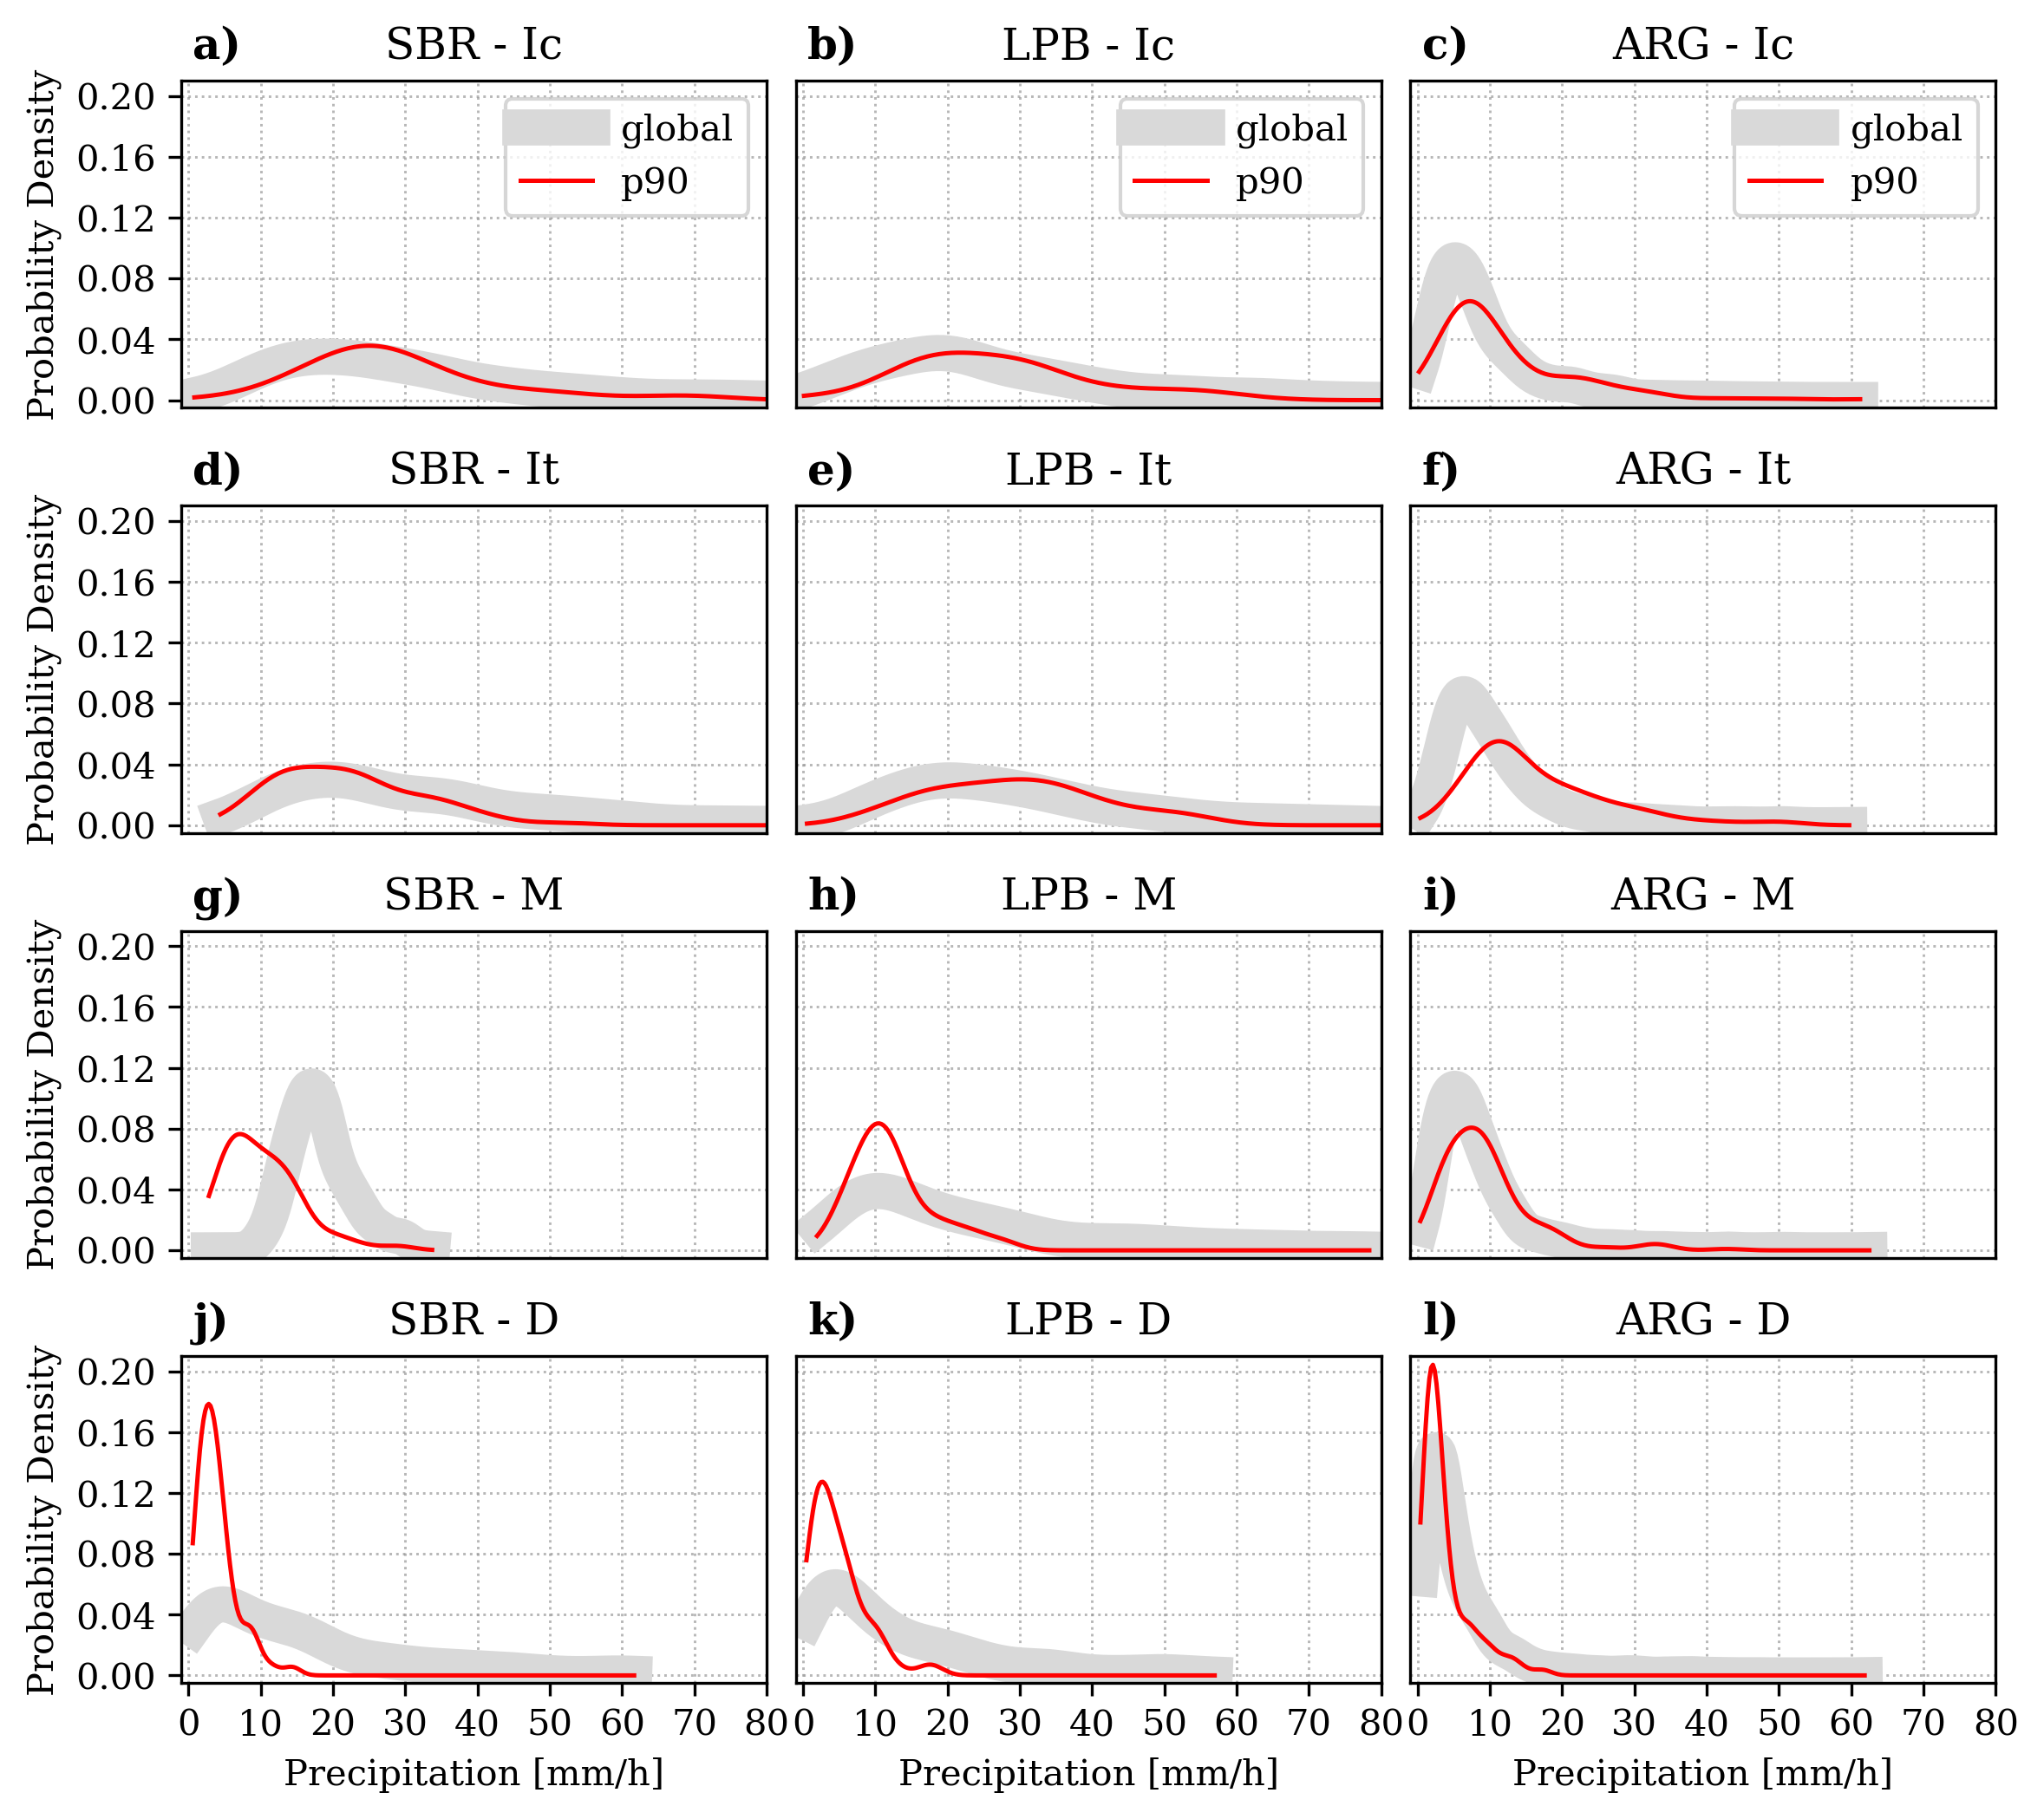
\includegraphics[width=\textwidth]{images/tp/PDF_tp_sigma025.png}
\caption[PDF de magnitudes máximas de precipitação total]{Funções de densidade de probabilidade (PDF, do inglês) para as magnitudes máximas de precipitação total (mm/h). As colunas indicam a região de ciclogênese (SBR, LPB, ARG) e as fileiras a evolução através das fases do ciclo de vida (Ic, It, M, D). Contrasta-se a população global (referência, sombreado cinza) com o subconjunto dos máximos de vorticidade relativa em 850 hPa alcançados em seu ciclo de vida: p90 (ciclones intensos, linha vermelha).}
\label{fig:pdf_tp}
\end{figure}

A Figura~\ref{fig:pdf_tp} mostra a distribuição estatística dos máximos espaciais de precipitação total (mm/h). 
Como fundamentam \citet{sinclair2023relationship}, os ciclones extratropicais são a causa principal da precipitação nessas latitudes, e compreender como a magnitude desta variável escala com a intensidade dinâmica do sistema é fundamental para avaliar o risco associado. 
Esses campos foram extraídos sistematicamente dentro do domínio lagrangiano centrado no núcleo de cada sistema, seguindo a mesma metodologia aplicada ao campo de vento (Capítulo~\ref{cap:resultados_wind10}). 
A População global encontra-se estratificada por região de ciclogênese (SBR, LPB, ARG) e o subconjunto de intensidade dinâmica definido segundo o pico máximo absoluto de vorticidade alcançado durante todo o ciclo de vida de cada ciclone (p90).

Nas fases de incipiência e intensificação (painéis a-f), SBR e LPB mostram distribuições amplas onde os ciclones intensos (p90) apresentam uma marcada tendência para maiores taxas de precipitação, com caudas que se estendem até os 60 mm/h. 
Como detalham \citet{chen2024evaluation}, a precipitação total resulta da soma da precipitação estratiforme em grande escala e a precipitação convectiva parametrizada, sendo esta última a que controla especificamente a cauda superior da distribuição. 
Em ambientes com maior disponibilidade de umidade e instabilidade estática como os que caracterizam SBR e LPB, o desenvolvimento dos ciclones mais intensos está intrinsecamente ligado a uma maior atividade convectiva \citep{sinclair2023relationship}. 
Por sua vez, esta convecção gera forçantes diabáticos que, como demonstram \citet{oertel2021warm} e \citet{blanchard2021warm}, propiciam as taxas de precipitação de alta intensidade a curto prazo responsáveis por engrossar o percentil superior ($p90$) durante as fases de desenvolvimento.

No entanto, ao alcançar a fase de maturidade (painéis g-h) e aprofundar-se para a decadência (painéis j-k), ocorre uma divergência estrutural: a curva do estrato p90 em SBR e LPB colapsa para a esquerda, desenvolvendo um pico modal sumamente estreito em valores mínimos de precipitação (entre 1 e 4 mm/h). 
Simultaneamente, a População Global retém distribuições muito mais estendidas e pluviosas centradas entre 15 e 20 mm/h. 
Por sua parte, a região de ARG (painéis c, f, i, l) manifesta um regime independente onde as distribuições permanecem em sua maior parte fortemente enviesadas para magnitudes baixas (moda em $\sim$5 mm/h), destacando-se uma dispersão ligeiramente maior para o $p90$ durante a intensificação e, na decadência (painel l), um colapso modal para valores mínimos ($\sim$2--3 mm/h) análogo, embora de menor magnitude, ao observado em SBR e LPB.
A disparidade nas caudas nesta variável revela forçantes ambientais regionais distintos que podem ser interpretados mediante um espaço de parâmetros ambientais. 
\citet{yanase2014parameter} sugerem que o desenvolvimento dos ciclones é altamente sensível às condições de umidade e baroclinicidade do ambiente, as quais definem a trajetória evolutiva do sistema. 
Nesse sentido, a identificação de precursores resulta vital; \citet{laurila2021characteristics} assinalam que os sistemas %(en el HN) 
que terminam gerando ventos e chuvas extremas possuem assinaturas dinâmicas distinguíveis desde suas etapas iniciais, embora a preditibilidade da precipitação máxima costuma ser menor que a do vento devido à sua natureza intermitente. 
Em nosso domínio, como demonstram \citet{russo2025impacts}, SBR e o limite com LPB apresentam fluxos de calor oceânico que sustentam a baroclinicidade e ancoram a convecção profunda. 
Este alargamento estatístico da precipitação na População Global acentua-se pela formação de ciclones durante todo o ano. A respeito disso, \citet{evans2012climatology} explicam que a vinculação com anomalias térmicas — as quais geram um ambiente de umidade e estabilidade na troposfera média — favorece a formação recorrente de ciclones com diversas estruturas térmicas no Atlântico Sul.
Dinamicamente, esta energia convectiva que alimenta o estrato extremo (p90) organiza-se mediante uma forte advecção quente e convergência de umidade: impulsionada pela Alta Subtropical em SBR, e por sua interação com o Jato de Baixos Níveis em LPB \citep{gramcianinov2024early}.

Em contraste, ARG apresenta precipitações marcadamente menores, refletindo um forçamento de latitudes altas caracterizado por baixa umidade absoluta e advecções frias e secas provenientes do Pacífico sul.
A assimetria nas distribuições pluviométricas reflete diretamente as condições do ambiente de gênese. 
Como assinalam \citet{gramcianinov2019properties}, os ciclones originados em ARG estão dominados pela baroclinicidade de latitudes médias, enquanto em LPB e SBR dependem fortemente da liberação de calor latente. 
Desde a energética atmosférica, \citet{coutodesouza2024thesis} corrobora esta dualidade ao demonstrar que os sistemas em ARG se sustentam na cadeia baroclínica clássica, em contraste com LPB e SBR, impulsionados ativamente pela cadeia baroclínica úmida de origem convectivo. 
Esta marcada diferença na disponibilidade de umidade e no forçamento diabático é o que explica fisicamente o viés positivo e as maiores taxas de precipitação observadas nessas regiões.

O desacoplamento entre a máxima intensidade dinâmica e a máxima precipitação durante a maturidade confirma a relação não linear entre a vorticidade e os forçantes da precipitação.
Desde uma perspectiva física, este comportamento revela que (p90) evoluem estruturalmente para sistemas profundos. 
Ao alcançar seu máximo, esses ciclones severos esgotam seu acesso à massa de ar úmido e instável transportada pela cinta transportadora quente (\textit{warm conveyor belt}), a qual é responsável pela convecção embebida mais intensa \citep{oertel2021warm, blanchard2021warm}. 
Em seu lugar, o núcleo experimenta uma pronunciada intrusão seca (\textit{dry intrusion}) induzida pela fratura frontal, um processo mediante o qual ar frio, subsidente e de baixa umidade proveniente da alta troposfera ou estratosfera se enrosca para o centro do sistema \citep{shapiro1999bridge}. 
% Esta dinámica suprime drásticamente la convección profunda en el dominio central. 
Este comportamento termodinâmico ao longo do ciclo de vida complementa a caracterização espacial de \citet{gramcianinov2019properties}, os quais confirmam que os ciclones originados em SBR e LPB concentram as taxas de precipitação mais intensas com uma marcada similitude entre ambas as regiões, enquanto os sistemas de ARG exibem uma natureza inerentemente mais seca, registrando uma menor quantidade de eventos que superem os 20 mm/dia.

A relação entre a vorticidade em 850 hPa do ciclone e os volumes máximos de precipitação exibe um comportamento não linear. 
Ao avaliar múltiplas medidas de intensidade, \citet{corner2025classification} evidenciam que as taxas pluviométricas se correlacionam moderadamente com a vorticidade em 850 hPa devido a mecanismos de retroalimentação onde o aquecimento diabático associado à chuva intensa gera anomalias de vorticidade potencial que reforçam a circulação em níveis baixos.
Esta eficiência termodinâmica sustenta as caudas pesadas de precipitação (superiores a 60 mm/h) observadas nas PDF do estrato $p90$ para SBR e LPB durante as etapas de intensificação, antes que o isolamento do núcleo corte o suprimento de umidade.
A quantificação deste comportamento estatístico invertido permite refutar empiricamente a hipótese de que a severidade do forçamento dinâmico (vorticidade máxima) se traduz invariavelmente em um incremento da chuva extrema ao longo de todo o ciclo de vida. 
Demonstrar que, no Atlântico Sul, os ciclones responsáveis pelos ventos mais destrutivos tendem a secar em seu núcleo durante a maturidade. 
As ameaças mais severas por chuvas associadas a ciclones intensos ($p90$) ocorrerão predominantemente durante as etapas precoces de gênese (incipiente) e intensificação, ou bem estarão associadas a sistemas de intensidade rotacional moderada cujas configurações termodinâmicas são mais eficientes para sustentar o ancoragem convectivo prolongado.

% ==============================================================================
% SECCIÓN PRINCIPAL: KDE ESPACIAL DE PRECIPITACIÓN
% ==============================================================================

\section{Distribuição espacial de máximos (KDE)}

\subsection{População Global}\label{subsec:kde_tp_global}

\begin{figure}[htbp]
\centering
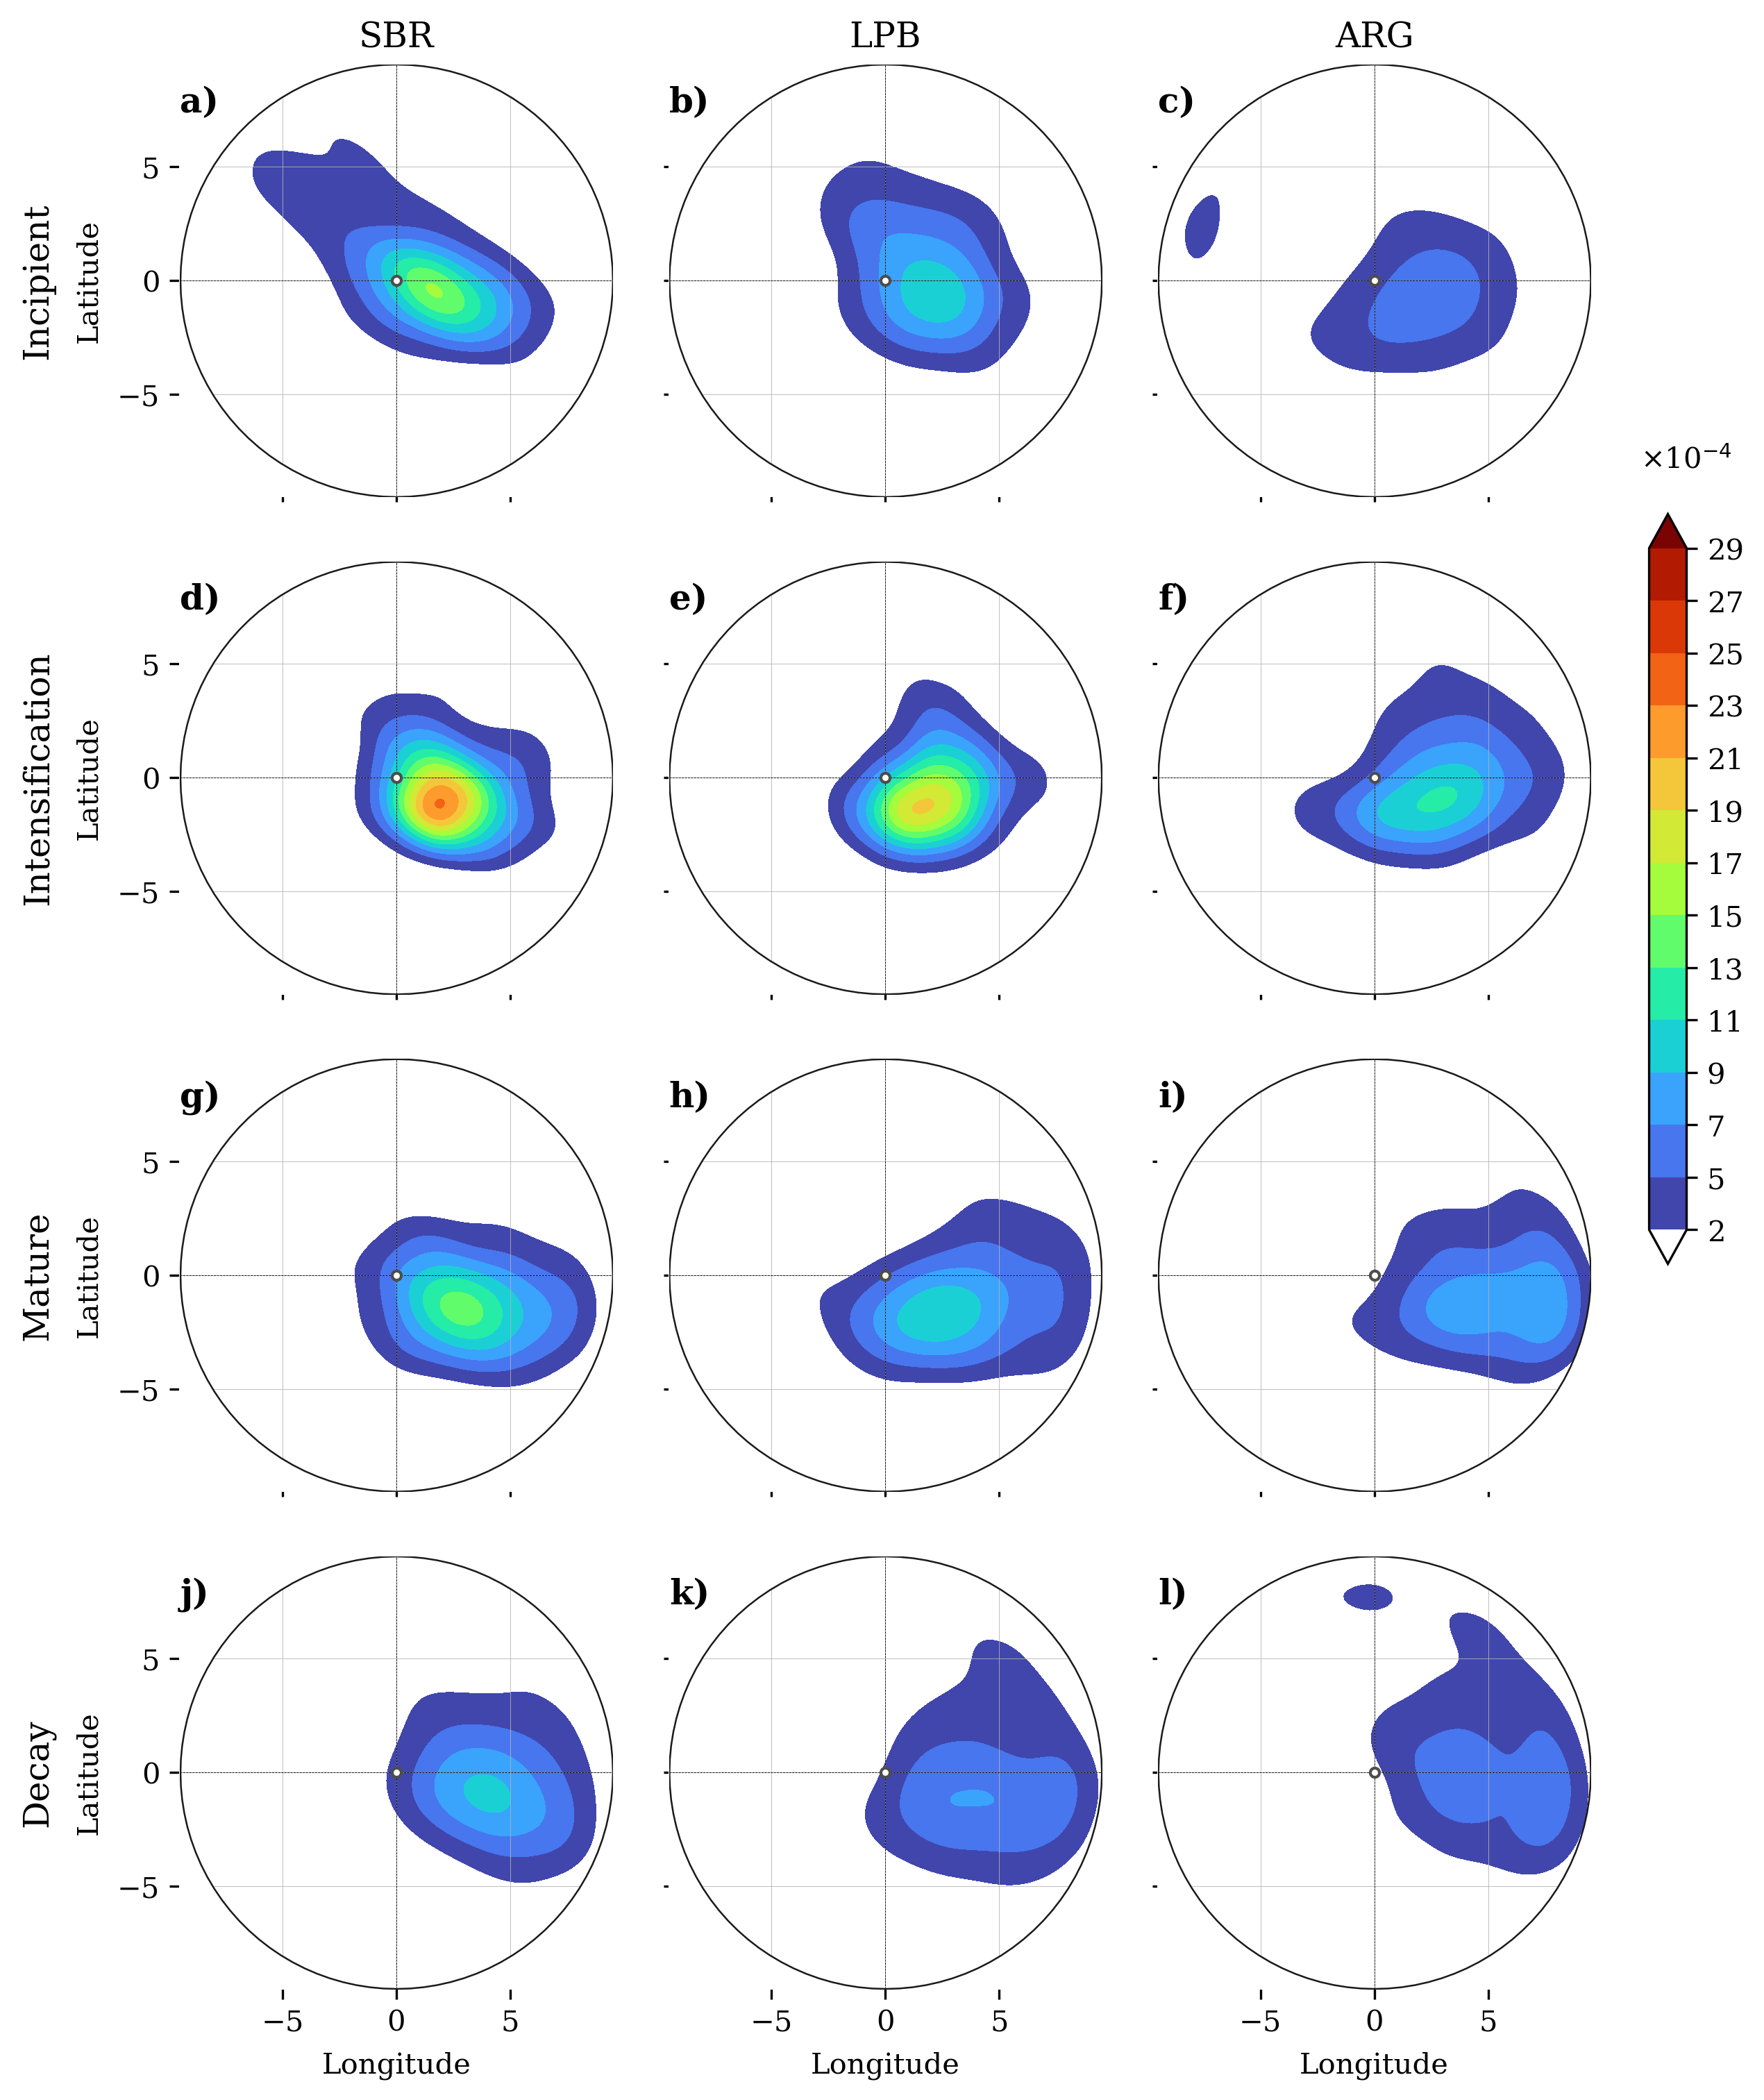
\includegraphics[width=\textwidth]{images/tp/kde_tp_global_fasesxreg.png}
\caption[Distribuição espacial (KDE) de precipitação máxima - População Global]{Estimação de densidade espacial bidimensional (KDE, do inglês) para a localização geométrica dos máximos de precipitação total (mm/h) na População Global de referência. A matriz organiza a evolução espacial através das fases evolutivas Incipiente (a-c), Intensificação (d-f), Maturidade (g-i) e Decadência (j-l), segregadas pelas regiões de ciclogênese SBR, LPB e ARG. O domínio lagrangiano abrange $20^{\circ} \times 20^{\circ}$ com centro no vórtice $(0,0)$. A barra de cores quantifica a densidade de probabilidade relativa escalada por $10^{-4}$.}
\label{fig:kde_tp_global}
\end{figure}

A Figura~\ref{fig:kde_tp_global} apresenta o campo probabilístico derivado da estimação de densidade por \textit{kernel} (KDE), o qual mapeia a localização espacial preferencial dos núcleos de precipitação máxima para a População Global dentro do marco de referência lagrangiano.
Diferentemente do campo de vento cuja distribuição incipiente já evidenciava certa difusão centrada no núcleo, a distribuição espacial da chuva máxima apresenta desde as etapas iniciais uma arquitetura fundamentalmente assimétrica em relação ao centro do ciclone.

A assimetria para o setor oriental e sudeste observada no KDE da População Global (Fig.~\ref{fig:kde_tp_global}, painéis a-f) emerge primariamente da arquitetura dinâmica da Cinta Transportadora Quente (WCB, do inglês). 

Segundo o modelo conceitual de \citet{browning1986conceptual} e as avaliações observacionais de \citet{naud2020evaluation}, a ascensão inclinada do WCB à frente do frente frio e acima do frente quente organiza a precipitação no flanco quente do ciclone, independentemente da região de gênese. 

Este forçante sinóptico explica a carga positiva consistente do EOF1 no quadrante sudeste (Fig.~\ref{fig:eof1_tp_global}) e constitui o esqueleto dinâmico universal da distribuição espacial. 
De fato, em escala global, \citet{catto2015front} demonstraram estatisticamente que existe uma vinculação inequívoca entre os WCBs, as frentes ativas e a ocorrência dos eventos de precipitação maiores em latitudes médias, justificando a concentração pluviométrica observada neste setor quente. 
Isto explica a carga positiva consistente do EOF1 no quadrante sudeste: no Hemisfério Sul, as condições de ascensão em grande escala acoplada a advecção de umidade satisfazem-se quase exclusivamente neste setor.

A orientação para o leste e sudeste das densidades máximas nas fases incipiente e intensificação (painéis a-f) reflete diretamente esta organização.
Sobre este esqueleto dinâmico do WCB, operam secundariamente moduladores regionais que explicam as diferenças de intensidade e extensão entre SBR, LPB e ARG. Em SBR e LPB, a configuração dos fluxos na camada limite reforça a assimetria oriental, como demonstram \citet{cardoso2022synoptic}, a circulação ciclônica induz anomalias positivas de convergência de umidade acopladas com advecção quente em níveis baixos, organizando a precipitação em bandas orientadas de noroeste a sudeste. 
Adicionalmente, o fluxo canalizado desde latitudes tropicais para o flanco leste do vórtice, documentado por \citet{vera2002cold}, atua como focos de convergência que intensificam a assimetria, resultando em núcleos de precipitação mais densos e estendidos no KDE (painéis a, b, d, e). 
Em contraste, para ARG, a maior distância à fonte de umidade tropical e a barreira orográfica dos Andes atenuam este fluxo, gerando um padrão mais difuso, menos intenso e com máximos deslocados para o nordeste (painéis c, f, i, l), onde a advecção zonal modificada pela topografia impõe uma organização distinta.

A robustez estatística deste padrão assimétrico na População Global, isto é, sua aparição consistente apesar da variabilidade intersistêmica deve-se ao contexto climatológico de gênese e trajetórias. 
A alta frequência de ciclogêneses nas imediações do norte da Argentina, Uruguai e sul do Brasil, junto com o deslocamento preferente para o sudeste sobre o oceano \citep{mendes2010climatology, simmonds2000mean}, assegura uma amostra onde o WCB interage sistematicamente com a configuração regional descrita.
Este trânsito constante de sistemas frontais maduros, caracterizado por frentes de avanço relativamente estáveis que varrem LPB e ARG, gera a huella dinâmica que captura o KDE espacial. 
No entanto, é crucial distinguir que este contexto climatológico não é um forçante físico direto da assimetria em um evento individual, mas um condicionante estatístico que garante a representatividade do padrão WCB-dominado na amostra global.

À medida que os sistemas transitam para a maturidade (M; painéis g-i) e a decadência (D; painéis j-l), esta assinatura espacial oriental expande-se e difunde-se, alargando a zona de probabilidade para o setor sudeste e sul, mas mantendo densidades de intervalo médio (tons verdes e celestes) que evidenciam a falta de um foco de convergência único nos ciclones ordinários.
Esta dispersão espacial do campo KDE e a perda de foco refletem a variabilidade estrutural intrínseca de um catálogo massivo: ao integrar os $N_{\text{global}}$ sistemas do catálogo incluindo ciclones fracos ou rasos que não logram uma estrutura frontal madura, o sinal espacial dilui-se. 
Caracterizar esta distribuição base é uma necessidade metodológica, já que permite estabelecer que, no ciclone médio, a precipitação concentra-se em seu setor oriental. 
A separação analítica dos sistemas mais severos (p90), abordada nas subseções seguintes, revela estruturas espaciais marcadamente distintas em relação a esta população de referência.

% ==============================================================================
\subsection{Subconjunto extremo (p90)}\label{subsec:kde_tp_p90}
% ==============================================================================

\begin{figure}[htbp]
\centering
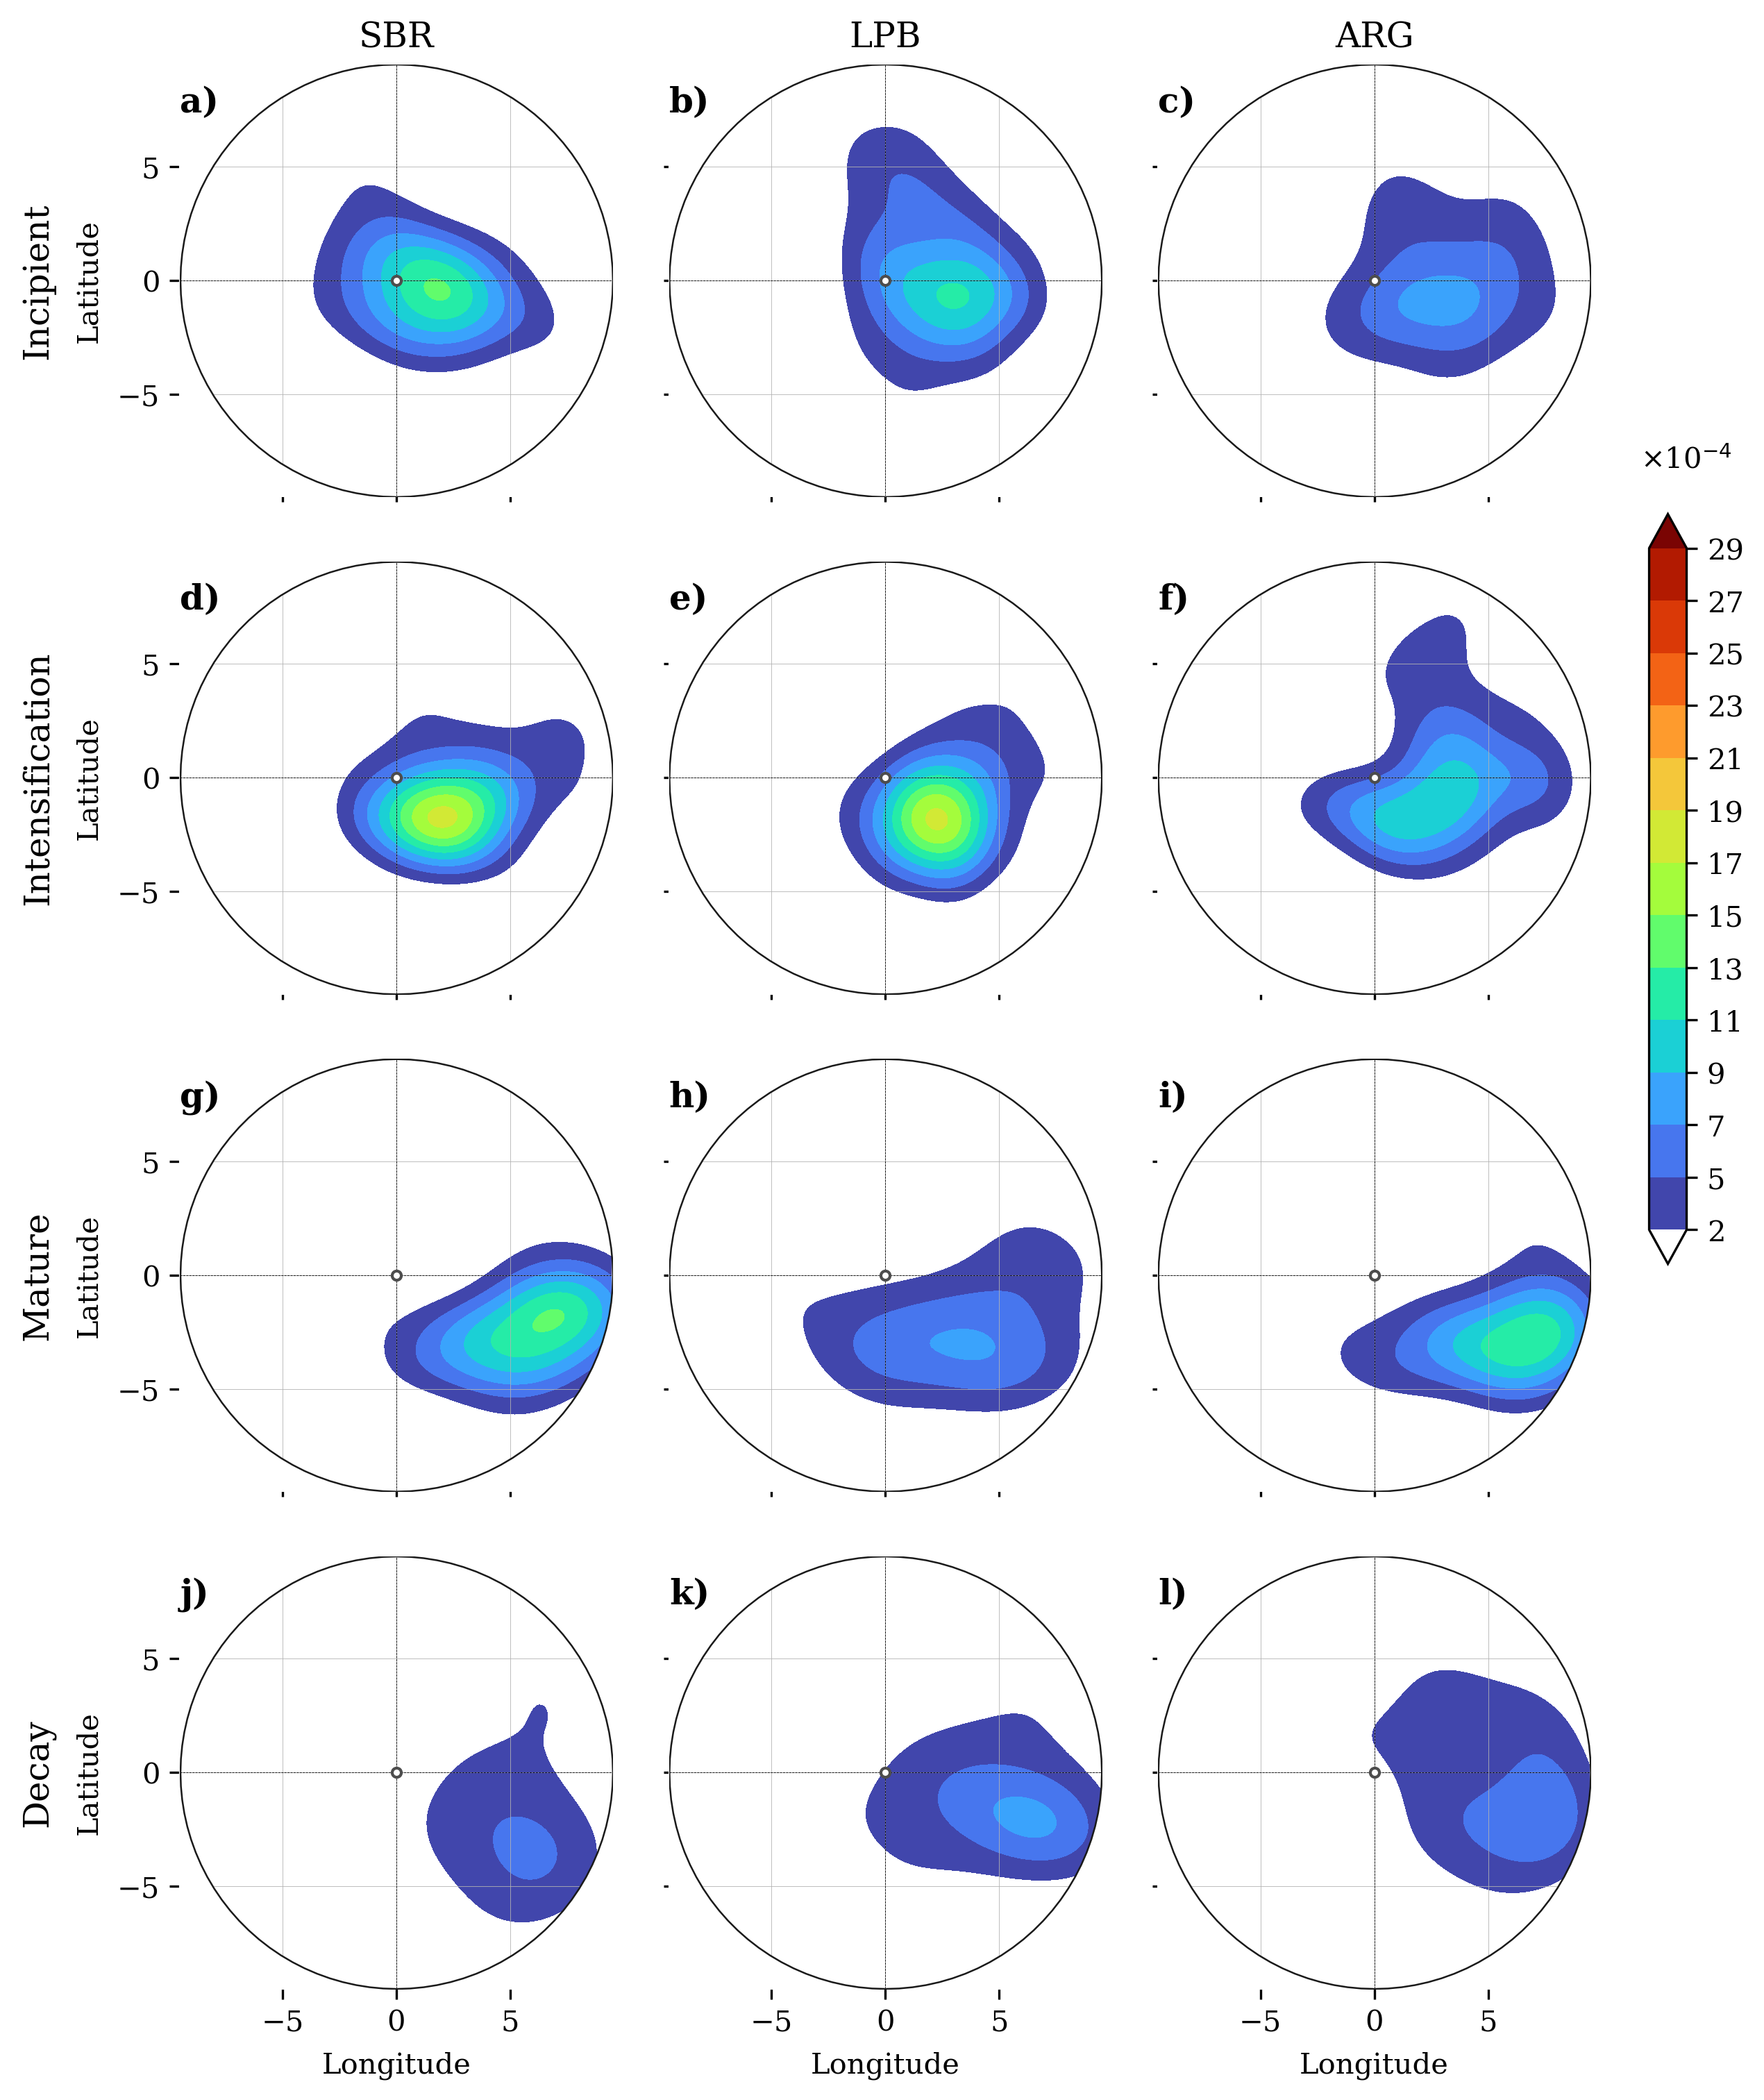
\includegraphics[width=\textwidth]{images/tp/kde_tp_p90_fasesxreg.png}
\caption[Distribuição espacial (KDE) de precipitação máxima - Subconjunto p90]{Estimação de densidade espacial bidimensional (KDE) para a localização geométrica dos máximos de precipitação total (mm/h) correspondente ao subconjunto de ciclones intensos (percentil 90). O formato dos painéis (a-l), a evolução temporal, a segregação regional e a escala cromática ($10^{-4}$) replicam a estrutura da Figura~\ref{fig:kde_tp_global}, permitindo quantificar o contraste com a população global.}
\label{fig:kde_tp_p90}
\end{figure}

Ao contrastar a distribuição base com o estrato de ciclones intensos (p90), a reorganização espacial resulta tão drástica quanto a observada no campo de vento, ainda que em sentido morfologicamente inverso. 
A Figura~\ref{fig:kde_tp_p90} revela que a arquitetura pluviométrica dos ciclones mais intensos não amplifica a concentração oriental da população geral, mas experimenta uma profunda mutação estrutural ao transitar para a maturidade (M; painéis g-i). 
As densidades máximas de precipitação afastam-se do centro de vorticidade $(0,0)$ e confinam-se em bandas sumamente estreitas e arqueadas. 
Nas regiões de SBR e LPB, essas zonas de alta probabilidade traçam uma geometria fortemente assimétrica que se concentra no setor leste e sudeste, estendendo-se para o sul do sistema, deixando o quadrante central e noroeste virtualmente desprovidos de máximos de chuva.

Esta reorganização espacial obedece primariamente ao processo de oclusão rápida própria de ciclones baroclínicos explosivos. 
Ao alcançar sua máxima intensidade, esses $p90$ experimentam uma violenta intrusão seca (\textit{dry intrusion}): o descenso forçado de ar frio e seco desde a alta troposfera penetra até o núcleo do ciclone, erradicando a nuvolosidade profunda e criando a característica cunha livre de chuva (\textit{dry slot}) nas imediações do centro \citep{shapiro1999bridge}. 
Simultaneamente, o fluxo ciclônico arrasta o remanescente de umidade da Cinta Transportadora Quente para a periferia, confinando-o estritamente no frente retrocedido (\textit{bent-back front}). 

Este processo gera a clássica banda de precipitação enroscada (\textit{wrap-around precipitation}), uma estrutura morfológica quase estacionária em relação ao centro de baixas pressões que explica a geometria arqueada observada no KDE durante a maturidade e a decadência \citep{schultz2021antecedents}. 
A formação desta banda periférica constitui a assinatura evolutiva culminante do modelo de Shapiro-Keyser, onde a seclusão quente isola termicamente o núcleo e reorganiza a umidade remanescente em uma estrutura de coma altamente previsível.
% Sobre esta geometría impuesta por la dinámica de oclusión, operan secundariamente mecanismos termodinámicos que determinan la intensidad extrema de la precipitación dentro de la banda enroscada. 
A concentração espacial dos volumes pluviométricos máximos responde a processos de subescala que mantêm taxas de condensação elevadas na periferia do sistema ocluído. \citet{priestley2022improved} destacam que a intensidade máxima das precipitações está estritamente condicionada pela força do WCB residual e pela presença de convecção profunda embebida ao longo do frente frio ou no núcleo do frente ocluído. 
Esta convecção embebida, documentada por \citet{oertel2021warm} e \citet{blanchard2021warm}, desencadeia correntes verticais velozes que incrementam drasticamente o conteúdo local de hidrometeoros mediante a liberação intensa de calor latente. 
% La retroalimentación diabática asociada inyecta masas de aire con baja vorticidad potencial en la tropopausa, alterando los gradientes térmicos e intensificando la circulación local, lo que sostiene rigidamente el patrón pluviométrico periférico frente a la intrusión seca central.

Em escala de processo, as taxas extremas pontuais dentro desta banda enroscada geram-se mediante circulações inclinadas de mesoescala (\textit{slantwise circulations}) associadas à cabeça de nuvem do frente ocluído. 
Como demonstram \citet{clark2005sting}, em eventos desenvolvidos sobre regiões de alta disponibilidade de umidade superficial como SBR e LPB, essas circulações ascendentes convectivas e baroclínicas geram condensação extremamente rápida. 
Esta retroalimentação termodinâmica local, impulsionada por instabilidades dinâmicas no entorno do frente retrocedido, justifica as densidades espaciais agudas e localizadas que dominam em $p90$, distinguindo esses sistemas da precipitação estratiforme moderada da População Global.

A consolidação e manutenção desta arquitetura singular dependem contextualmente dos forçantes de superfície do Atlântico subtropical. 
Os intensos fluxos de calor latente e sensível desde o oceano para a atmosfera, modelados por \citet{gozzo2013air} para ciclones tipo Shapiro-Keyser nesta região, aquecem a baixa troposfera e sustentam a convecção na vizinhança do frente retrocedido. 
Complementarmente, \citet{andrade2024composite} assinalam que a advecção de ar frio e seco sobre águas quentes potencializa a evaporação e os fluxos de calor latente. Este vapor, ao condensar-se, libera calor latente que intensifica a circulação e organiza movimentos verticais ascendentes nas áreas de maior precipitação.
% Estos flujos oceánico-atmosféricos actúan como condicionantes necesarios que permiten cuando ocurre un ciclon intenso (p90), aunque no determinan por sí solos la geometría la precipitación, que es inherente a la dinámica de oclusión.

De acordo com o marco conceitual de \citet{zscheischler2018future}, no hemisfério norte, os perigos meteorológicos surgem da combinação de múltiplos processos físicos interagindo a diferentes escalas. 
Por isso, a quantificação desta arquitetura espacialmente desacoplada fornece informação nova no Atlântico Sul. 
Nas regiões SBR e LPB, os núcleos do subconjunto $p90$ representam a superposição espaço-temporal de: 
(i) a convergência sinóptica induzida pelo ciclone ocluído, 
(ii) o forçante de mesoescala de convecção embebida na banda enroscada, e 
(iii) a fonte de umidade oceânica que sustenta a condensação. 
Esta configuração implica que, em ciclones intensos maduros, os forçantes destrutivos operam em quadrantes opostos: enquanto as rajadas de vento mais severas se hiperconcentram no setor noroeste (associadas à CCB), os máximos remanescentes de chuva são empurrados para o sudeste e sul, orbitando a margem exterior da intrusão seca. 
Este achado revela que o epicentro do perigo associado a precipitações e o epicentro do perigo eólico em eventos severos não colidem geograficamente, mas impactam de maneira defasada e nos ciclones intensos.

% Este hallazgo exige una reestructuración de los sistemas de alerta temprana multicomponente, confirmando que el epicentro del peligro hidrológico y el epicentro del peligro eólico en eventos severos no colisionan geográficamente, sino que impactan de manera desfasada y en regiones espaciales mutuamente excluyentes.

% ==============================================================================
% SECCIÓN: PATRONES DOMINANTES DE VARIABILIDAD (EOF) - PRECIPITACIÓN
% ==============================================================================
\section{Organização estrutural: Análise EOF}\label{sec:eof_tp}
\subsection{Fracionamento de variância}\label{subsec:var_exp_tp}
% ==============================================================================

\begin{figure}[htbp]
\centering
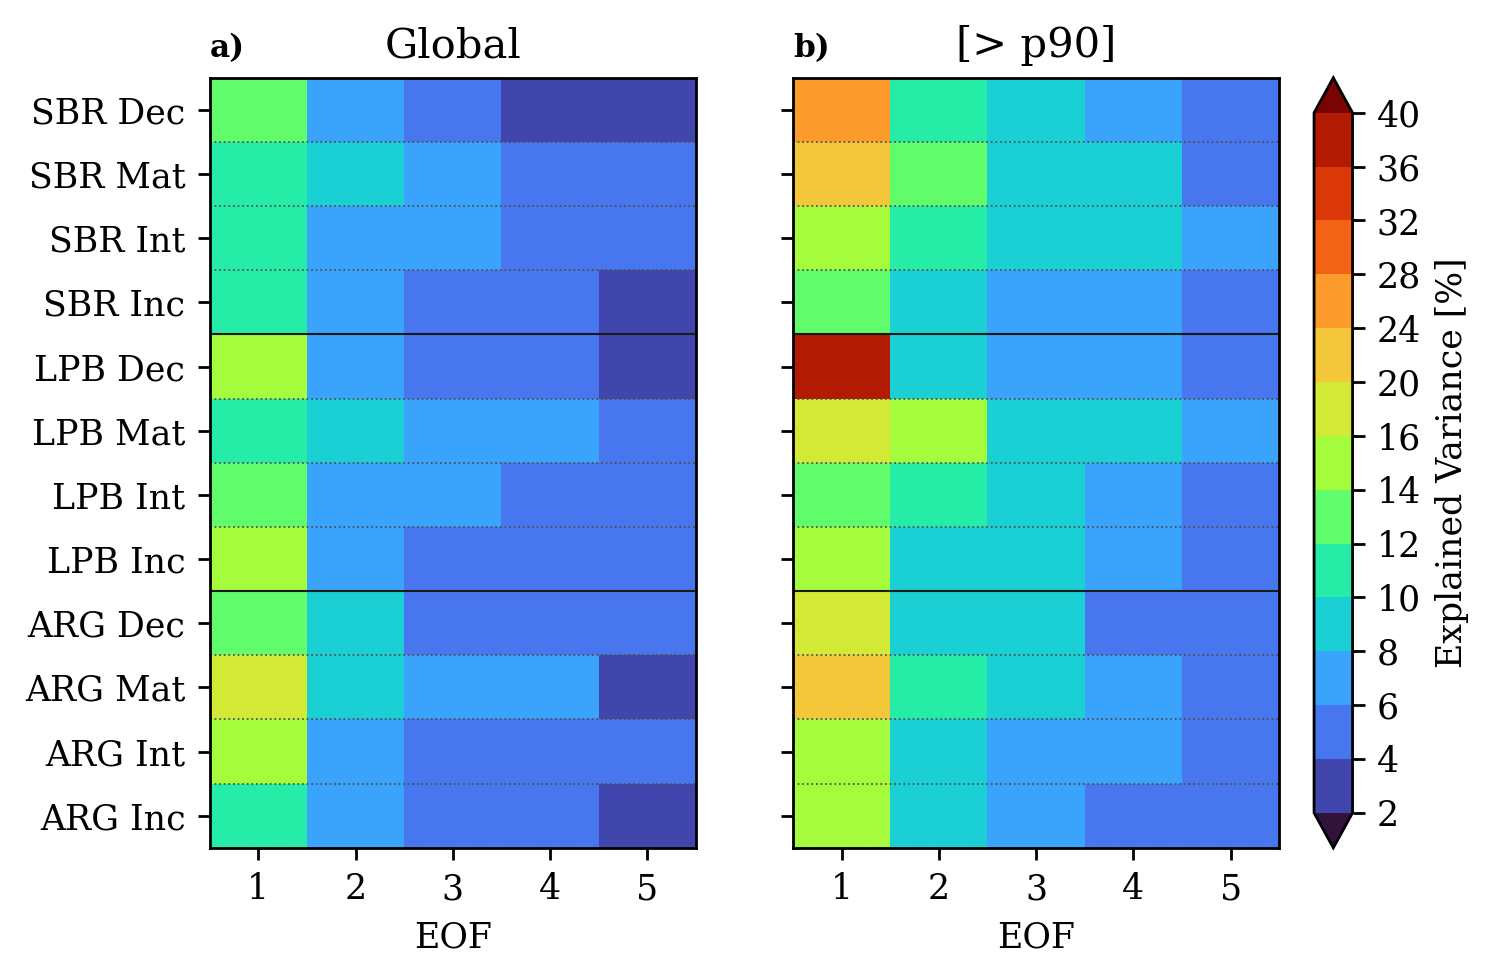
\includegraphics[width=0.8\textwidth]{images/tp/all_expvar_tp_mean2times.png}
\caption[Variância explicada pelos primeiros cinco modos (EOF1--EOF5) de precipitação]{Fracionamento da variância espacial total contida nos primeiros cinco modos dominantes (EOF1 a EOF5) do campo de precipitação total. Contrasta-se a distribuição da variância da População Global frente ao subconjunto de intensidade (p90) ao longo do ciclo de vida para cada região de ciclogênese.}
\label{fig:var_exp_tp}
\end{figure}

A Figura~\ref{fig:var_exp_tp} apresenta a distribuição percentual da variância espacial explicada por cada um dos cinco primeiros modos empíricos (PC1 a PC5). 
As colunas contrastam a População Global (painel a) contra os subconjuntos de intensidade extrema (p90, painel b). 
As fileiras correspondem às doze combinações de região de ciclogênese (SBR, LPB, ARG) e fase evolutiva (incipiente, intensificação, maturidade e decadência). 
A escala cromática quantifica o percentual de variância explicada, onde os tons azuis e verdes indicam baixa concentração de variância (modos dispersos) e os tons amarelos e vermelhos revelam alta concentração no modo principal.

Visualmente, o contraste entre painéis é marcado: enquanto a População Global (a) exibe predominantemente tons frios distribuídos uniformemente entre os cinco modos, o painel de sistemas intensos (b) mostra tons quentes concentrados na primeira coluna (PC1) durante as fases finais do ciclo de vida.
Especificamente, na decadência de LPB e SBR, o PC1 alcança valores superiores a 35\% e 25\% respectivamente, enquanto na População Global esses mesmos casos mal superam os 10\%. Esta transição cromática de frio a quente no estrato p90 constitui a evidência visual do colapso dimensional que caracteriza os ciclones intensos em sua fase final.

A análise desta distribuição revela um padrão marcadamente distinto ao observado nas variáveis cinemáticas. Enquanto no vento o modo dominante concentra a maior parte da variabilidade, na precipitação a variância distribui-se de maneira aplanada entre múltiplos modos durante as fases incipiente, intensificação e maturidade da População Global.
Este comportamento disperso contrasta abruptamente com o salto observado nos ciclones intensos (p90) ao ingressar na fase de decadência, onde o EOF1 alcança 36,5\% em LPB e 26,2\% em SBR, superando com folga os valores típicos da climatologia geral (entre 11\% e 16\%).

O aplanamento generalizado do espectro de variância na precipitação responde à natureza espacialmente descontínua deste campo. 
Diferentemente das variáveis de massa (geopotencial), que obedecem a gradientes contínuos de grande escala, a chuva está governada por frentes ativas de escala muito reduzida, núcleos de convecção embebida e taxas assimétricas de liberação de calor latente \citep{oertel2021warm}. 
Esta fragmentação espacial implica que nenhum único padrão espacial pode capturar a diversidade de configurações pluviométricas presentes na amostra. 
De acordo com os critérios de interpretação EOF estabelecidos por \citet{hannachi2007empirical}, a distribuição da variância entre múltiplos modos indica que o campo pluviométrico é inerentemente heterogêneo, exigindo a retenção de vários modos ortogonais para reconstruir adequadamente a variabilidade observada. 
Nesse sentido, \citet{graf2017objective} revelam que a ciclogênese não opera em categorias discretas, mas em um contínuo físico onde os processos úmidos e a produção diabática de vorticidade potencial constituem dimensões de variabilidade quase independentes, o que explica a dispersão da energia entre EOF2 e EOF5 durante as fases iniciais em todas as regiões.

O comportamento distintivo dos ciclones intensos (p90) durante a decadência, onde o EOF1 concentra até 36,5\% da variância em LPB, obedece à consolidação da banda enroscada \textit{wrap-around precipitation} como estrutura dominante. 
Quando os ciclones severos alcançam a fase final de seu ciclo de vida, a intrusão seca e o frente retrocedido organizam a precipitação remanescente em uma geometria espacial rigidamente coerente e quase estacionária em relação ao centro do vórtice. 
Esta organização estrutural reduz drasticamente a heterogeneidade espacial que caracteriza os sistemas moderados, permitindo que um único modo espacial capture a configuração pluviométrica dominante. 
Como assinalam \citet{hannachi2023eof}, a análise EOF permite examinar sistemas complexos mediante a decomposição de sua matriz de covariância espacial, e neste caso particular, a consolidação da banda periférica durante a decadência gera uma redução dimensional efetiva onde o primeiro modo retém a maior fração possível da variância total do campo.

As diferenças regionais no fracionamento de variância refletem a influência dos forçantes orográficos e térmicos estacionários do Hemisfério Sul.
De acordo com \citet{inatsu2004zonal}, a gênese e o desenvolvimento do trem de ondas baroclínicas apresentam uma marcada assimetria zonal, forçada pela interrupção do fluxo que supõe a cordilheira dos Andes e pelos contrastes térmicos mar-terra. 
Esta modulação dinâmica em grande escala fixa zonas preferenciais de ciclogênese e áreas recorrentes de frontogênese, o que explica que regiões como ARG ou oeste de LPB apresentem valores ligeiramente superiores de variância explicada pelo EOF1 durante as fases iniciais em relação a SBR, onde a influência oceânica e a convecção tropical introduzem maior variabilidade estrutural.
Desde uma perspectiva metodológica, a técnica EOF resulta apropriada para esta análise porque transforma o conjunto de dados atmosféricos interdependentes em novas variáveis espacialmente ortogonais desenhadas para capturar a máxima fração possível da variância total em cada modo sucessivo \citep{wilks2019statistical_ch13}. 
Embora na População Global esta variância fique distribuída entre vários modos, a decomposição permite isolar a resposta dominante do sistema em relação às anomalias estruturais de menor escala. 

Esta confirmação quantitativa resulta metodologicamente necessária. 
Revela que o impacto pluviométrico em sistemas ordinários é difuso, justificando a necessidade de reter múltiplos modos espaciais para sua descrição completa. 
No entanto, também prova que os $p90$ possuem a capacidade singular de organizar as precipitações remanescentes em geometrias coerentes ao final de seu ciclo de vida, fenômeno que não tem equivalente nos campos de vento e que constitui uma assinatura distintiva dos sistemas severos do Atlântico Sul.

% ==============================================================================
\subsection{Padrões espaciais dominantes (EOF1)}\label{subsec:eof1_tp}
% ==============================================================================

\subsubsection{População Global}\label{subsubsec:eof1_tp_global}

\begin{figure}[htbp]
\centering
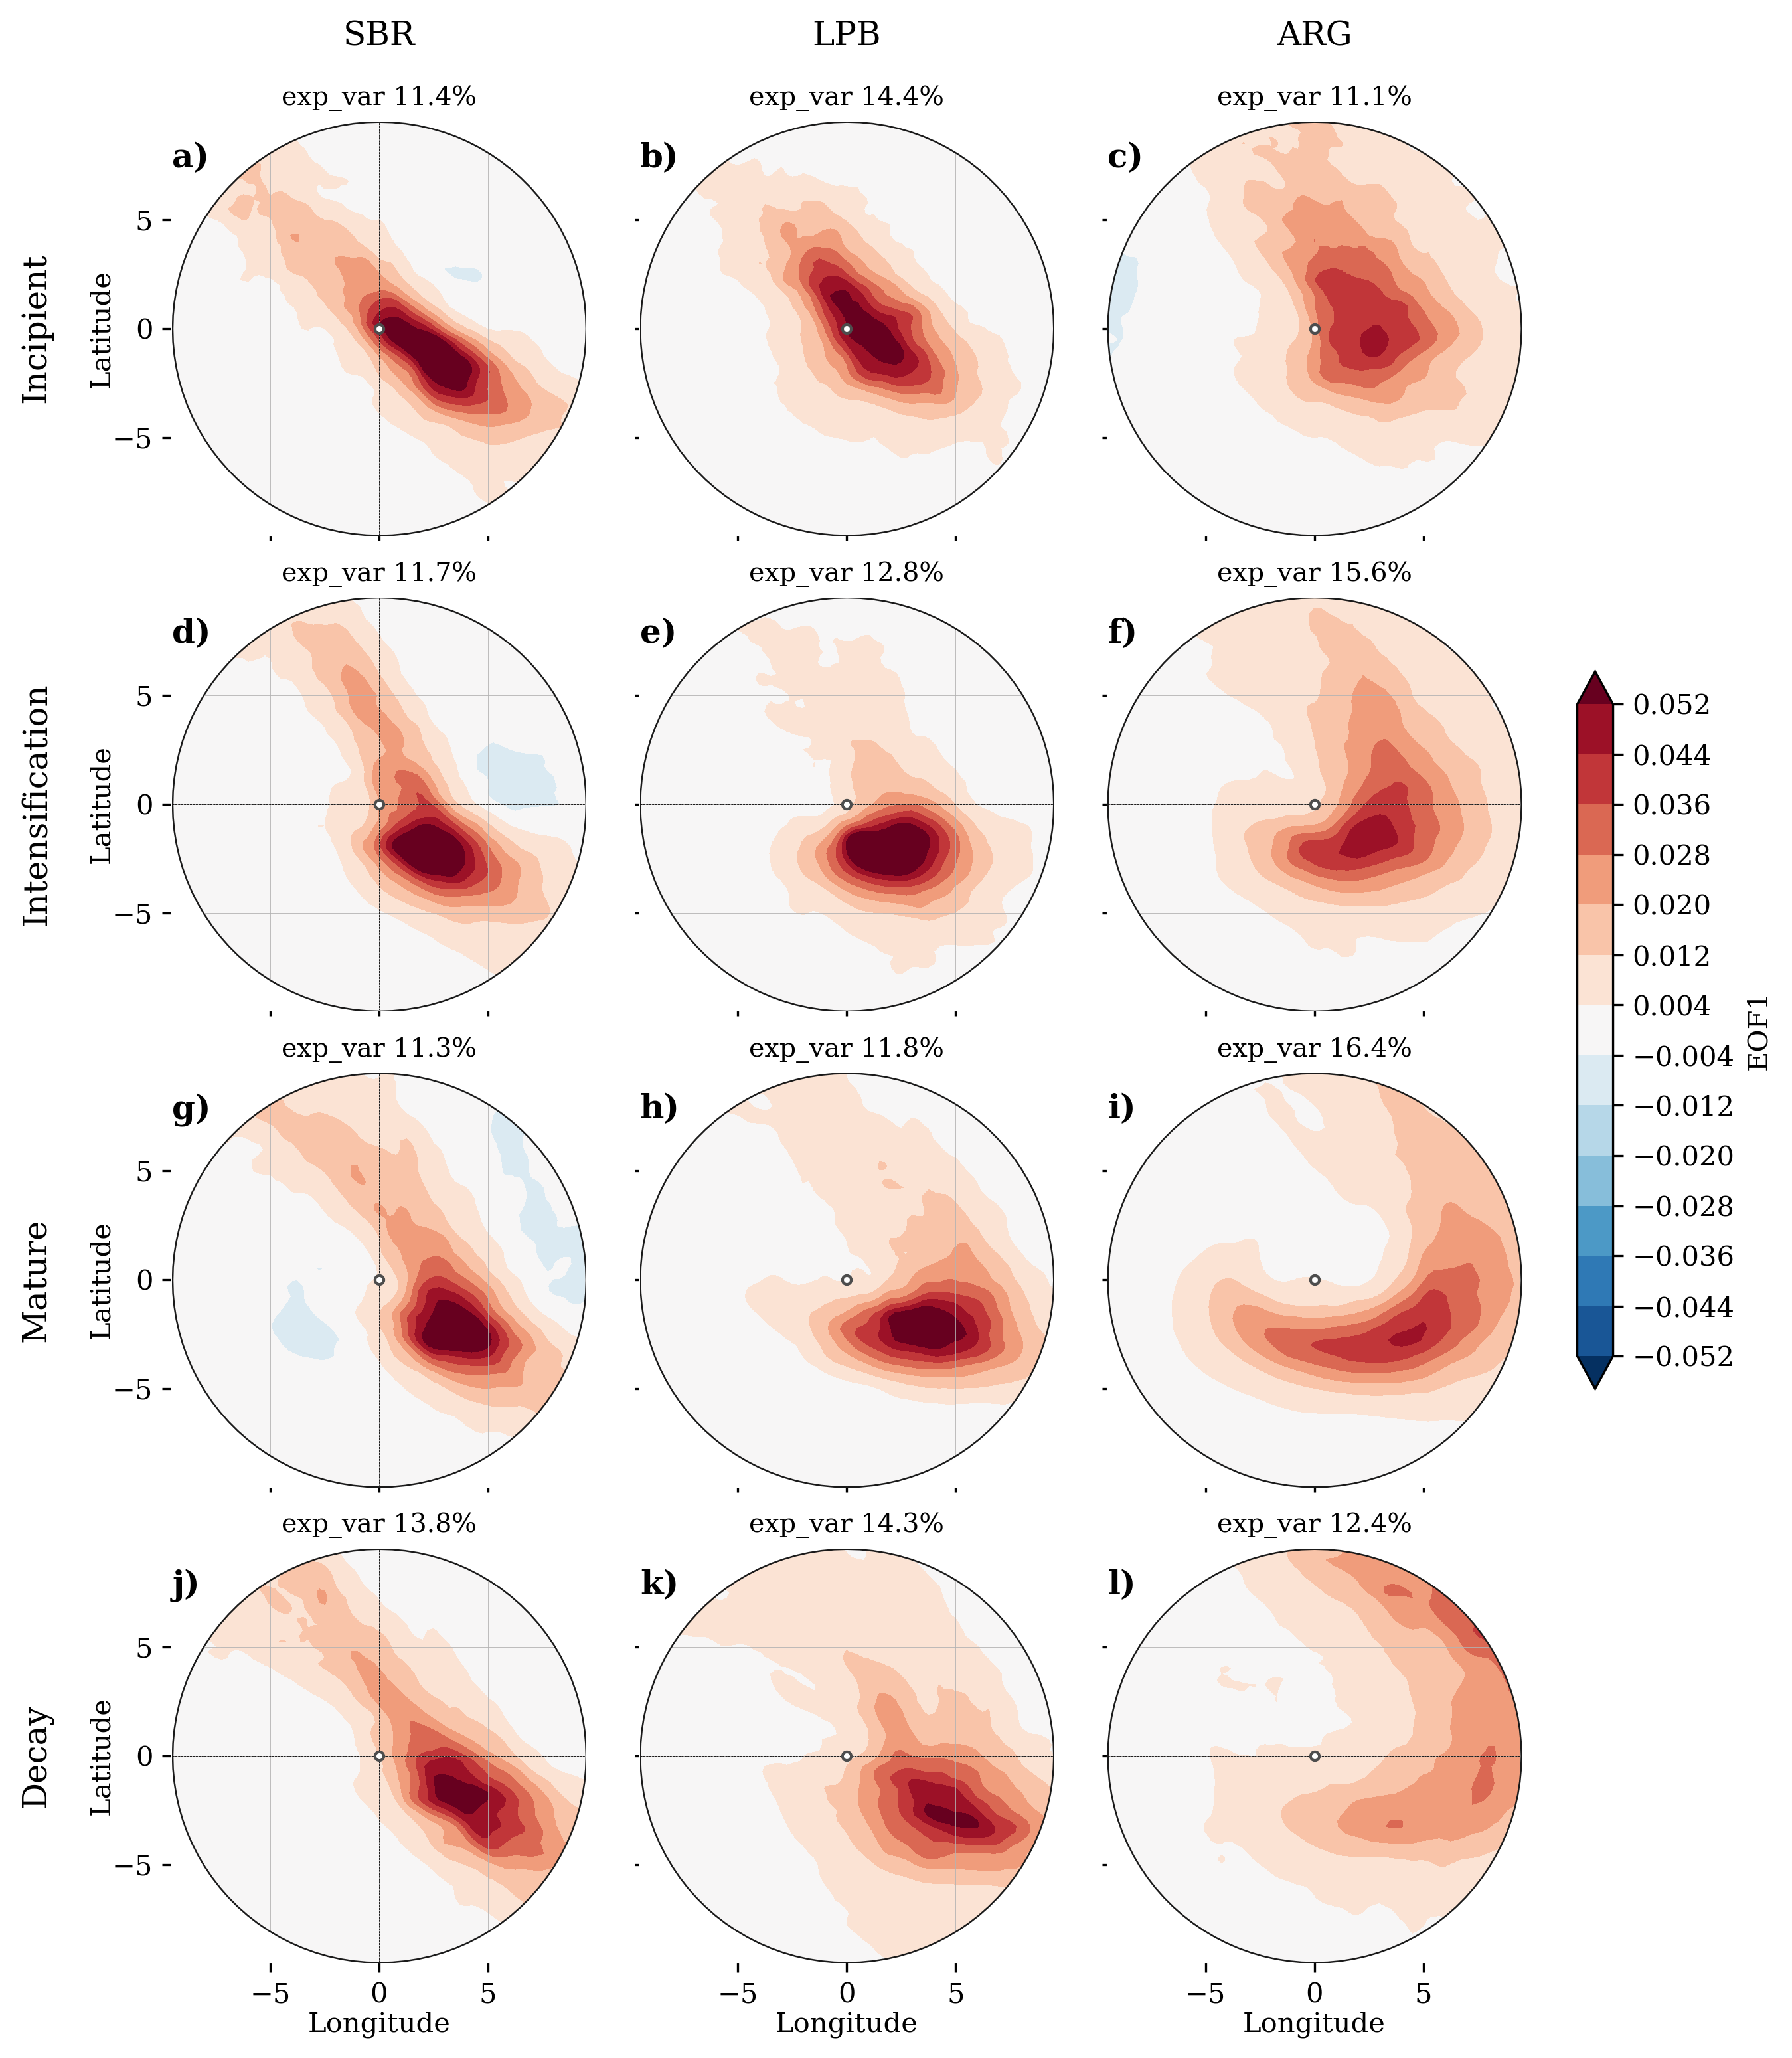
\includegraphics[width=\textwidth]{images/tp/pca1_tp_global_fasesxreg.png}
\caption[EOF1 de precipitação total - População Global]{Primeiro modo espacial (EOF1) da precipitação total (mm/h) para a População Global de referência. A disposição matricial organiza a evolução por regiões de ciclogênese em colunas (SBR, LPB e ARG) e as fases de desenvolvimento evolutivo em fileiras (Incipiente, Intensificação, Maturidade e Decadência). Sobre cada painel indica-se o percentual da variância espacial total explicada (\textit{exp\_var}) por esta componente principal. A escala cromática divergente quantifica as anomalias estruturais relativas ao centro do vórtice.}
\label{fig:eof1_tp_global}
\end{figure}

A Figura~\ref{fig:eof1_tp_global} apresenta os padrões espaciais correspondentes ao primeiro modo empírico (EOF1) da precipitação total, seguindo a mesma disposição matricial de 4 fileiras (fases) por 3 colunas (regiões) empregada nos campos KDE previos. 
Cada painel mostra um domínio circular lagrangiano de 20 graus centrado no vórtice (ponto branco), com contornos de cores que representam as anomalias estruturais de precipitação em relação à média. 
Diferentemente do padrão observado no EOF1 do vento a 10 metros (Seção~\ref{subsubsec:eof1_wind10_global}), aqui o modo dominante exibe uma organização marcadamente assimétrica: as anomalias positivas (tons avermelhados) concentram-se preferentemente no setor oriental e sudeste do domínio, enquanto os valores negativos (tons azuis) aparecem de maneira fragmentada e de menor magnitude. 
Os percentuais de variância explicada anotados em cada painel oscilam entre 11,1\% e 16,4\%, confirmando visualmente a baixa dominância do primeiro modo em relação à variável de vento a 10 metros. 
Esta distribuição irregular, com contornos difusos reflete a natureza inerentemente descontínua do campo pluviométrico.

O padrão espacial observado obedece primariamente à organização dinâmica da Cinta Transportadora Quente (WCB). 
Segundo o modelo conceitual de \citet{browning1986conceptual}, a ascensão inclinada do WCB à frente do frente frio e acima do frente quente organiza inerentemente a precipitação no flanco quente do ciclone. 
No contexto do Atlântico Sudoeste, este fluxo termodinâmico obrigatório configura o esqueleto espacial base que se observa nas três regiões: uma banda de anomalias positivas orientada de noroeste a sudeste, coincidente com a trajetória do ar ascendente no setor quente do sistema. 
A variabilidade capturada pelo EOF1 representa, portanto, as flutuações na intensidade e posição desta corrente ascendente à medida que o ciclone evolui.

Sobre este esqueleto dinâmico do WCB, operam moduladores regionais que explicam as diferenças na intensidade do padrão entre SBR, LPB e ARG. 
A disponibilidade de umidade para alimentar o WCB está condicionada pelo transporte remoto de vapor de água desde o Atlântico tropical para as zonas baroclínicas ativas. 
De acordo com \citet{gozzo2017climatology}, a ciclogênese no Atlântico Sudoeste está profundamente supeditada a este aporte de umidade remota, somada aos fluxos locais de calor latente por evaporação sobre a superfície oceânica. 
Esta configuração explica por que o padrão do EOF1 em SBR e LPB apresenta anomalias mais intensas e concentradas perto da costa ocidental, onde a convergência de umidade é máxima, enquanto em ARG o padrão é mais difuso e deslocado para o nordeste.

O mecanismo físico que explicaria o sinal positivo da EOF1 reside nos padrões de circulação dos baixos níveis da troposfera. 
Como documentam \citet{rocha2016estudo}, a convergência em 850 hPa estimula a ciclogênese no Atlântico Sul. 
Esta convergência facilita um transporte constante de umidade desde regiões como a Amazônia, o qual se concentra na zona de formação do sistema em SBR e LPB. 
A coincidência espacial entre a variabilidade da EOF1 e as áreas de convergência identificadas pelo autor sugere uma resposta à eficiência deste transporte de umidade e à liberação de calor latente que aporta para a precipitação neste setor do ciclone.

A distribuição espacial capturada pelo EOF1 reflete a natureza intermitente e localizada inerente aos processos convectivos de precipitação. 
Como assinalam \citet{naud2020evaluation}, a convecção no setor quente organiza-se em regiões de ascensão dinâmica e de convergência de umidade. 
Nesta região, a intensidade da precipitação está estreitamente vinculada à força de dita ascensão, o que gera núcleos de precipitação que contrastam marcadamente com as áreas livres de precipitação ou de garoa dispersa no resto do ciclone. 
Por outro lado, desde uma perspectiva estatística, \citet{hannachi2007empirical} explicam que a baixa variância explicada pelo primeiro modo se deve, precisamente, ao caráter altamente variável do campo analisado. 
No caso específico da precipitação, esta limitação na variância é esperável, já que a análise EOF frequentemente tem dificuldades para capturar eficientemente processos físicos não lineares que são, por natureza, localizados e intermitentes.

A extração deste modo univariado para a climatologia geral confirma que, em um cenário médio, as flutuações pluviométricas carecem de uma simetria centralizada duradoura e são regidas pela variabilidade transitória do setor frontal oriental.

Estabelecer esta linha de base dispersa permite dimensionar objetivamente a magnitude da transformação estrutural que experimentam os eventos severos (p90), os quais, ao alcançar a maturidade e ocluir-se, abandonam este comportamento transitório para confinar a precipitação em geometrias rigidamente estruturadas, como se examina a seguir.
 
\subsubsection{Subconjunto p90}\label{subsubsec:eof1_tp_p90}
% 
\begin{figure}[htbp]
\centering
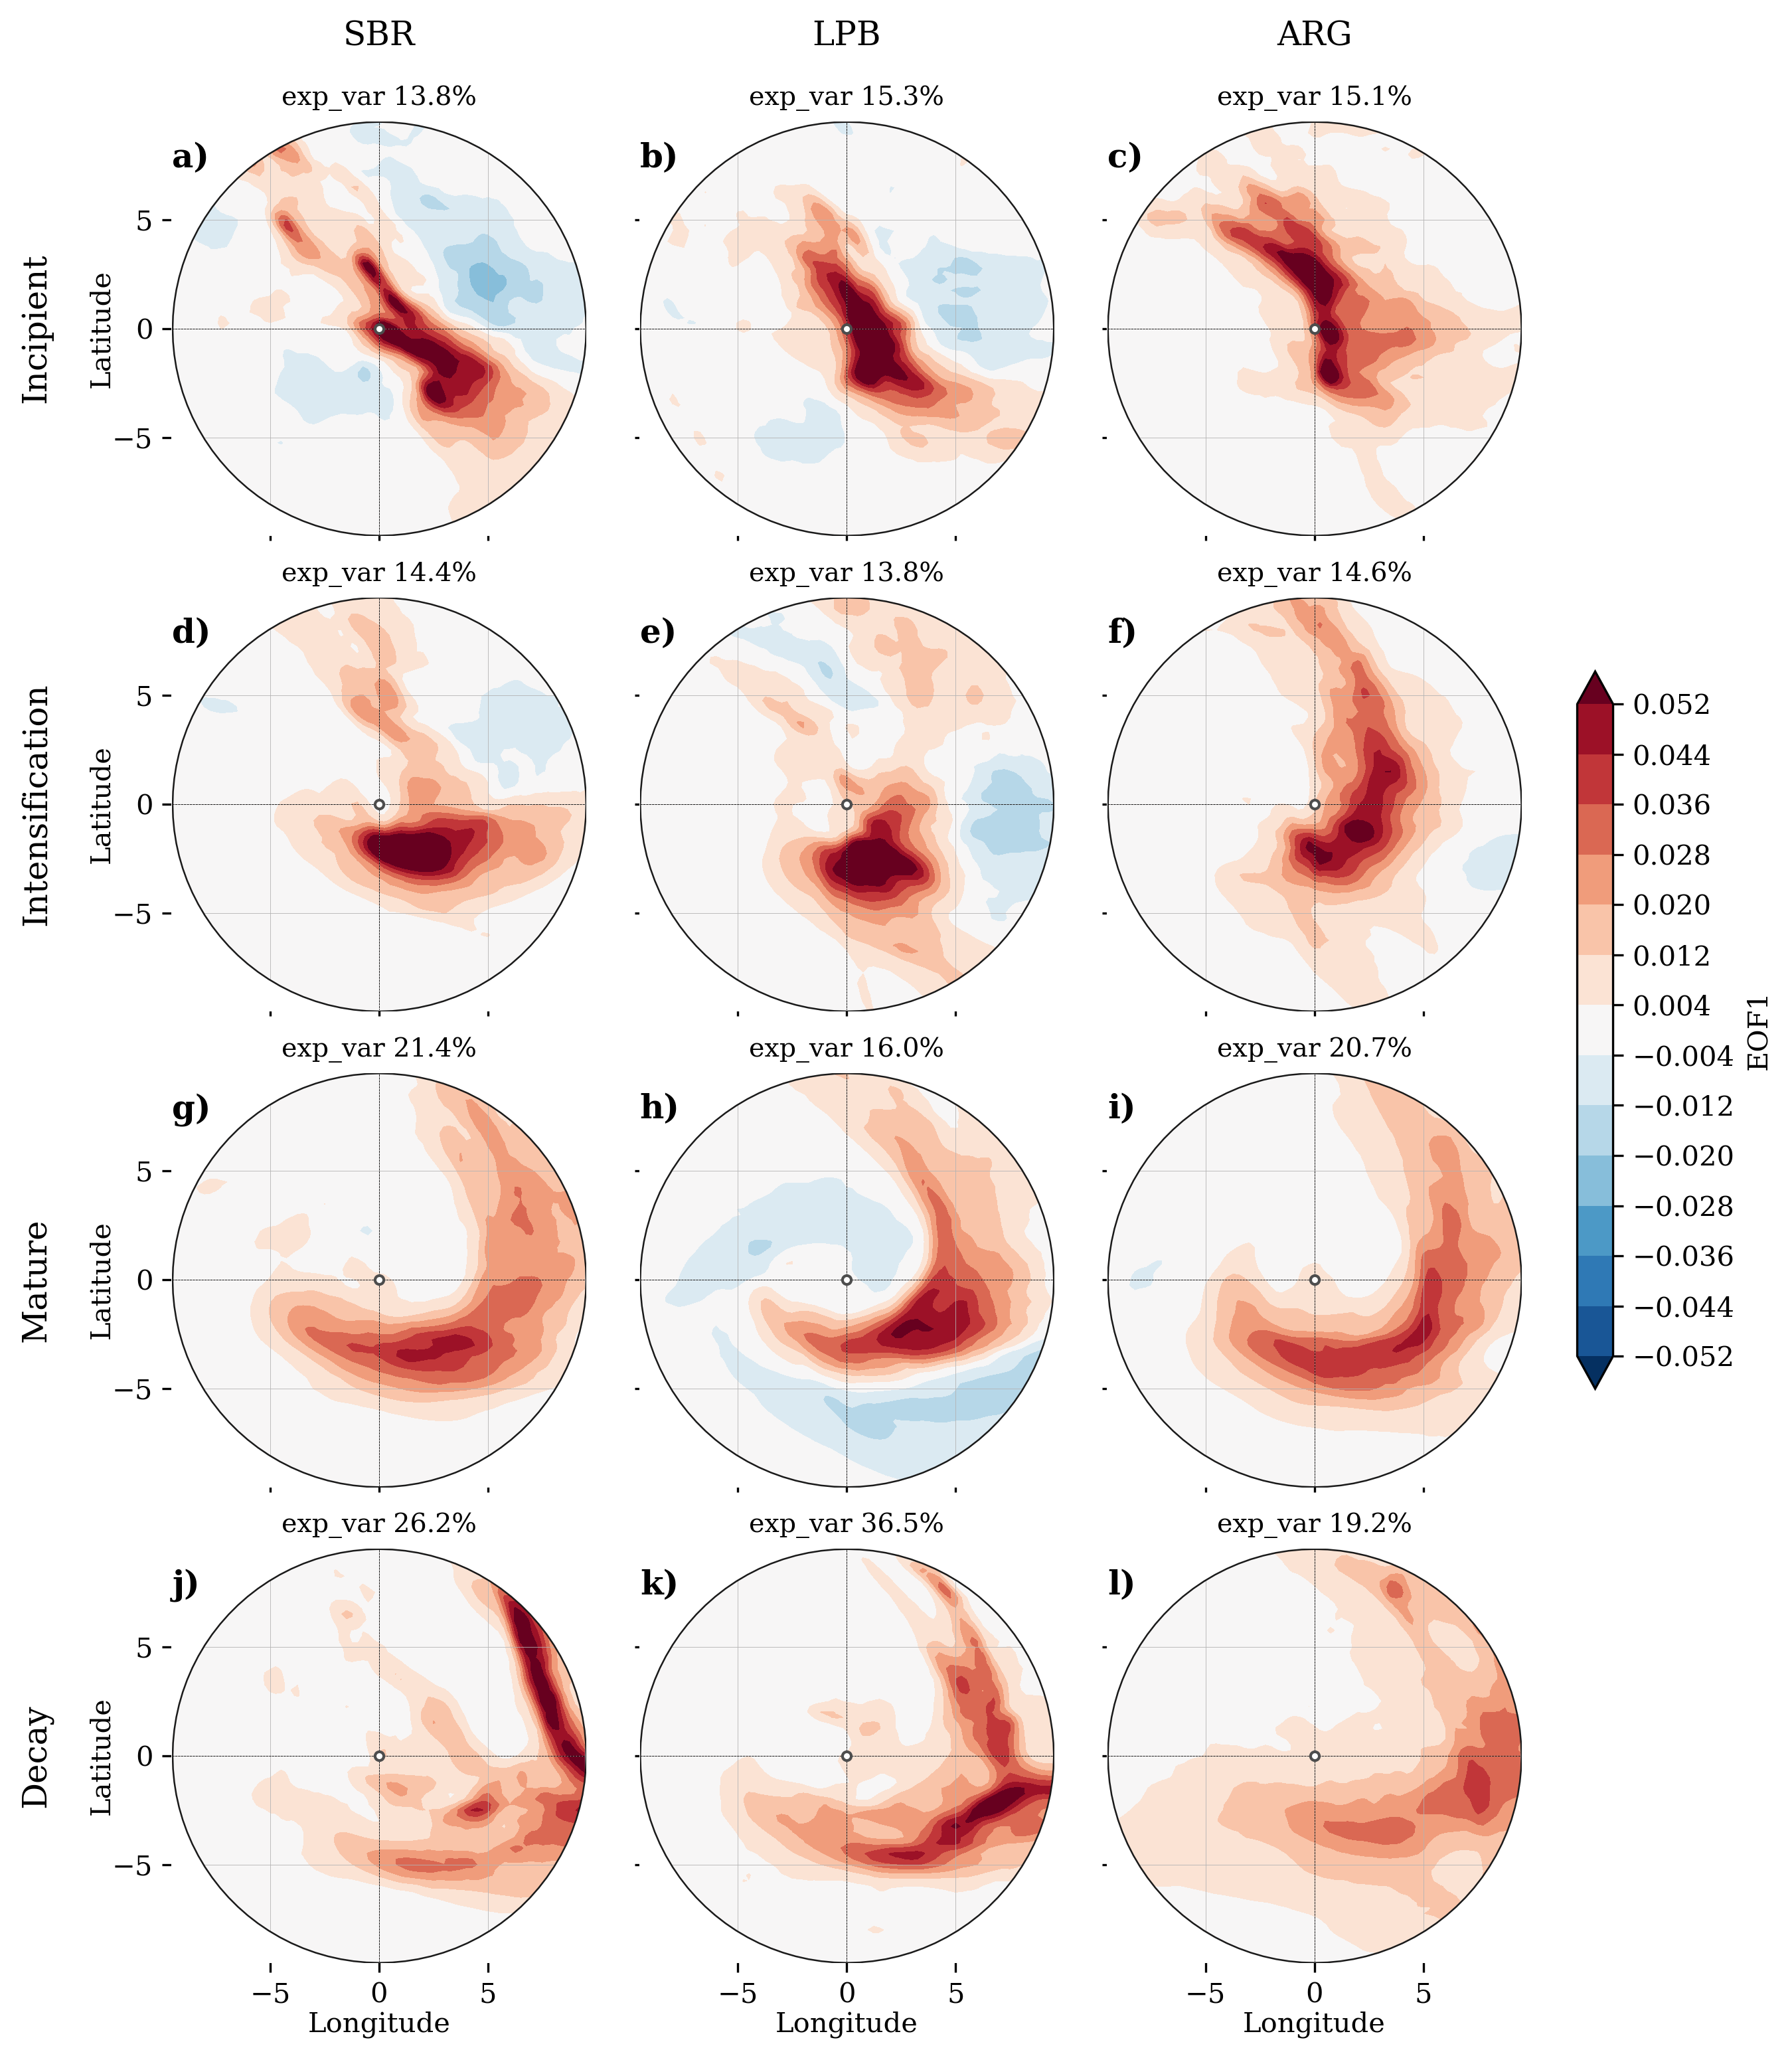
\includegraphics[width=\textwidth]{images/tp/pca1_tp_p90_fasesxreg.png}
\caption[EOF1 de precipitação total - Subconjunto p90]{Primeiro modo espacial (EOF1) da precipitação total (mm/h) para o estrato de ciclones intensos (percentil 90). O formato dos painéis (a-l), a nomenclatura de variância explicada e o domínio espacial mantêm uma correspondência estrita com a Figura~\ref{fig:eof1_tp_global}, permitindo quantificar a profunda transformação estrutural que experimentam os sistemas severos, especialmente durante sua oclusão final.}
\label{fig:eof1_tp_p90}
\end{figure}

A Figura~\ref{fig:eof1_tp_p90} apresenta os padrões espaciais do primeiro modo empírico para o estrato de ciclones intensos, mantendo a disposição matricial de doze painéis utilizada na população global. 
O contraste visual com a Figura~\ref{fig:eof1_tp_global} é imediato: enquanto na população geral os valores de variância explicada oscilavam entre 11\% e 16\%, aqui observa-se um salto quantitativo nas fases finais, alcançando 21,4\% em SBR Maturidade, 36,5\% em LPB Decadência e 26,2\% em SBR Decadência. 
Morfologicamente, durante as fases de incipiência e intensificação (painéis a-f), o EOF1 mantém padrões irregulares ancorados ao setor oriental, similares embora mais intensos que os da população global. 
No entanto, ao transitar para a maturidade e a decadência (painéis g-l), produz-se uma reorganização estrutural: o padrão caótico é substituído por uma assinatura geométrica nítida e coerente. 
Em SBR (painel j), esta assinatura consiste em uma banda anômala arqueada que se concentra no setor sudeste e estende-se para o sul do vórtice; em LPB (painel k), a estrutura positiva é mais ampla e envolve o sistema desde o nordeste até o sudeste, com uma leve anomalia negativa no centro-sul. 
Em ambas as regiões, o quadrante central e noroeste fica virtualmente livre de anomalias positivas. 
Esta configuração assimétrica, especialmente evidente durante a decadência, contrasta marcadamente com a dispersão difusa observada nos sistemas moderados.

A emergência desta estrutura espacialmente coerente obedece primariamente ao processo de oclusão severa própria do modelo de Shapiro-Keyser. 
A forte deformação cinemática do vórtice força uma intrusão seca profunda desde a alta troposfera que aniquila a convecção no centro geométrico do sistema, criando a característica cunha livre de precipitação. 
Simultaneamente, o remanescente de umidade da Cinta Transportadora Quente é arrastado pela intensa circulação ciclônica para a periferia, ficando confinado estritamente no frente retrocedido \citep{shapiro1990life, schultz2021antecedents}. 
Esta reorganização gera a banda de precipitação enroscada \textit{wrap-around precipitation}, uma estrutura morfologicamente quase estacionária em relação ao centro de baixas pressões que explica a geometria arqueada observada no EOF1 durante as fases finais. 
Dado que esta banda concentra taxas de precipitação muito superiores a seu ambiente seco e mantém uma posição relativamente estável em relação ao vórtice, a análise EOF a identifica como a fonte dominante de variância espacial, justificando o salto abrupto no percentual de energia capturada pelo primeiro modo.

A localização específica e a intensidade desta banda enroscada dependem secundariamente das condições termodinâmicas da superfície oceânica subjacente. 
A disponibilidade de umidade forçada pela Temperatura da Superfície do Mar e a presença de núcleos de forte ascensão sinóptica modulam a capacidade do sistema para sustentar a condensação extrema na periferia do ciclone ocluído. 
Como demonstram \citet{laureanti2024relation} ao examinar eventos severos sobre o leste e centro do Brasil mediante análise EOF, os extremos pluviométricos não são fenômenos isolados, mas estão estritamente ligados aos fluxos locais de calor latente desde o oceano para a atmosfera. 
Estes fluxos aquecem a baixa troposfera e retroalimentam as correntes verticais, ancorando geograficamente as áreas de máxima variância e permitindo que a banda enroscada alcance as taxas de precipitação extremas observadas no estrato p90, particularmente sobre SBR e a bacia atlântica adjacente onde o contraste térmico oceânico é mais pronunciado.

A manutenção desta arquitetura assimétrica durante a decadência responde adicionalmente a processos de retroalimentação diabática internos. 
A intensa liberação de calor latente dentro da banda de precipitação periférica fomenta o isolamento térmico do núcleo ciclônico. 
De acordo com \citet{reboita2022from}, este aquecimento diabático reduz o cisalhamento vertical do vento e facilita o alinhamento entre os sistemas de níveis baixos e altos, consolidando a seclusão quente e desacoplando a dinâmica pluviométrica das flutuações lineares do gradiente sinóptico de fundo. 
Este processo assegura que a banda enroscada não seja um fenômeno transitório, mas uma estrutura que persiste enquanto o ciclone se dissipa.

Estas transformações estruturais podem situar-se dentro do marco conceitual do ciclo de vida ciclônico. 
Tal como sugerem \citet{hart2003cyclone}, o desenvolvimento de um ciclone pode ser avaliado mediante transições de fase que parametrizam a assimetria da espessura relativa e a estrutura térmica do núcleo (frio vs. quente). 
No contexto de nossas regiões de estudo, o passo para a maturidade e decadência em ciclones intensos implica necessariamente o desenvolvimento de seclusões quentes que ditam a localização dos forçantes frontogênicos. 
No entanto, é preciso distinguir que este marco descreve o contexto evolutivo geral, enquanto a forma específica da banda enroscada observada no EOF1 deriva diretamente dos processos de oclusão e dos forçantes oceânicos descritos precedentemente.

A extração desta assinatura estrutural assimétrica e rígida constitui o fechamento analítico das variáveis individuais. 
Ao contrastar estes padrões com os campos de vento equivalentes (Seções~\ref{subsubsec:eof1_wind10_p90}), evidencia-se geometricamente o desacoplamento espacial das ameaças: enquanto a variabilidade das rajadas destrutivas compacta-se no quadrante noroeste (governada pela cinta transportadora fria), a chuva remanescente organiza-se em uma ferradura sólida nos quadrantes sudeste e sul. 

% Este hallazgo valida la necesidad de evaluar los ciclones oceánicos como fenómenos de riesgo compuesto desfasado, donde el epicentro del peligro hidrológico y el epicentro del peligro eólico operan en regiones espaciales mutuamente excluyentes, y provee el respaldo teórico para avanzar hacia el análisis acoplado de ambas variables en el capítulo siguiente.

% ==============================================================================
\subsection{Significância estatística}\label{subsec:significancia_tp}
% ==============================================================================

Para discriminar entre sinais físicos robustos e flutuações próprias da reamostragem, avaliou-se a significância estatística dos autovetores espaciais mediante o método Bootstrap-$t$ (Seção~\ref{subsec:bootstrap_significancia}). 
A Figura~\ref{fig:xeof_madurez_global_tp} documenta os três primeiros modos (EOF1--EOF3) e suas respectivas séries temporais (PC1--PC3) para a População Global em fase de maturidade, enquanto a Figura~\ref{fig:xeof_madurez_p90_tp} apresenta a análise equivalente para o subconjunto p90. 
O achurado delimita as áreas onde as cargas espaciais resultaram estatisticamente significativas a 95\% de confiança.

\begin{figure}[htbp]
\centering
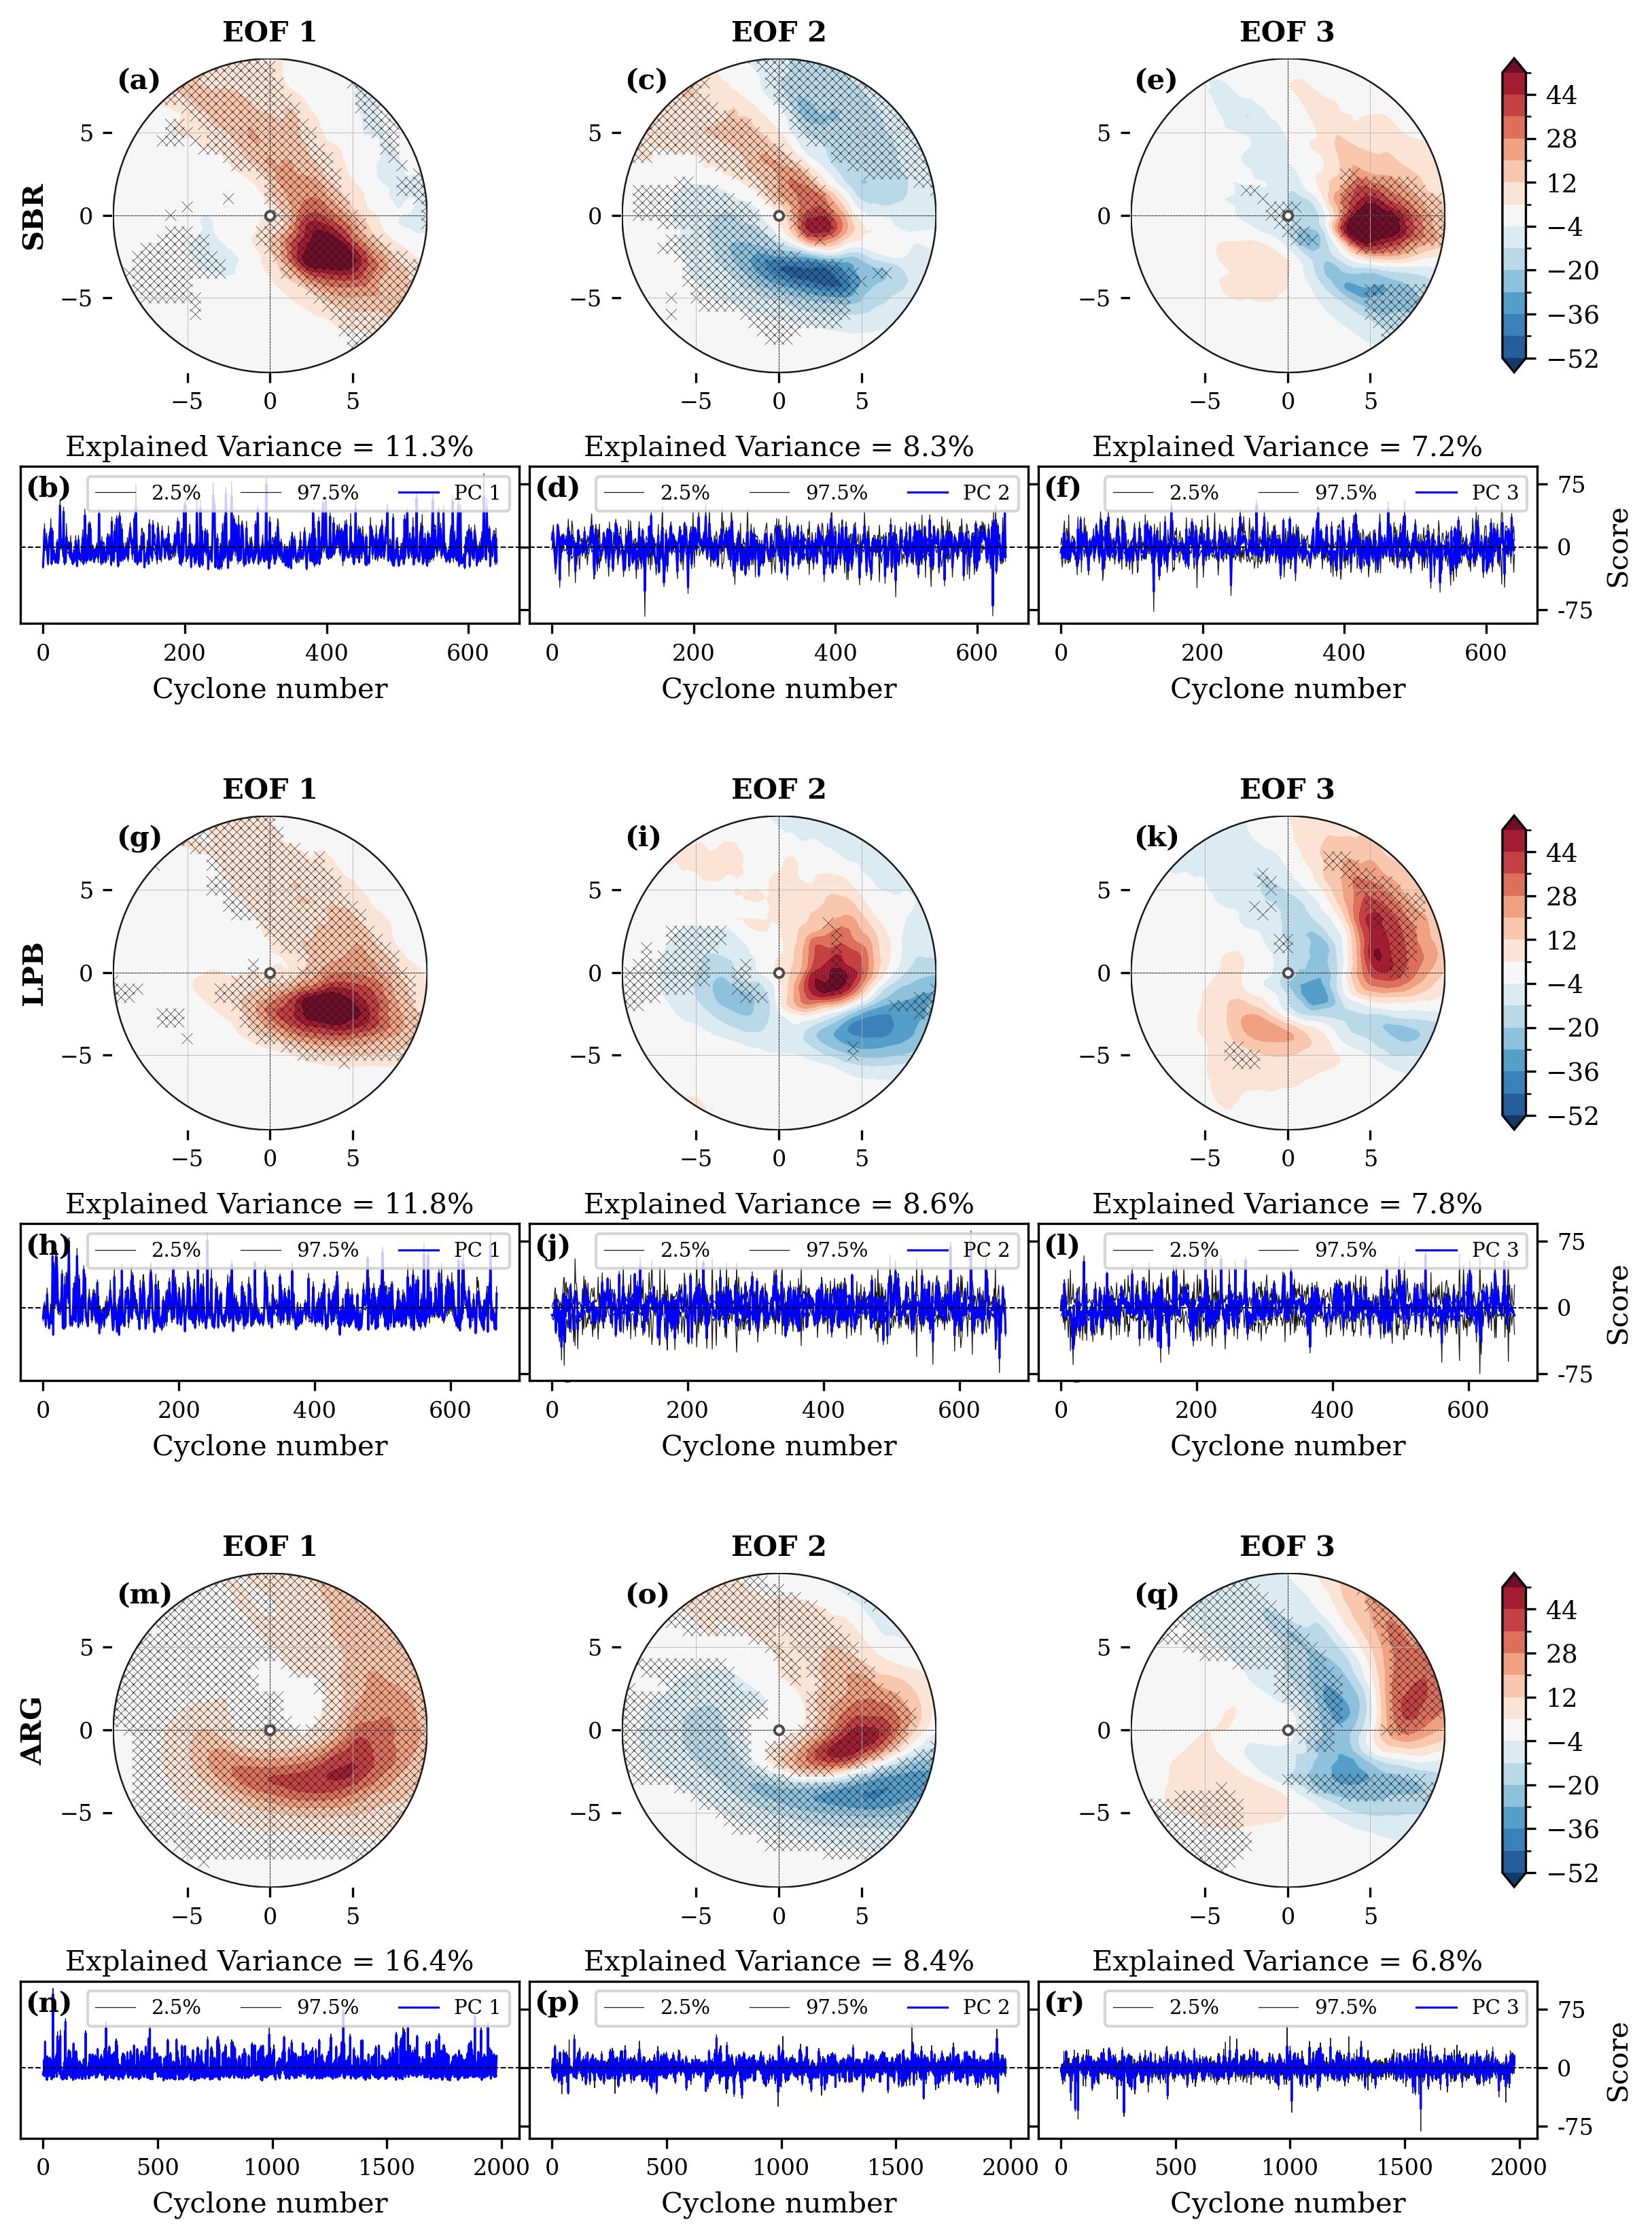
\includegraphics[width=\textwidth]{images/tp/xeof_global_tp_mature.png}
\caption[Significância espacial dos EOFs em fase de maturidade - População Global (tp)]{Decomposição EOF da precipitação total para a População Global em fase de maturidade. Painéis (a, c, e): mapas dos três primeiros modos espaciais (EOF1--EOF3) com achurado indicando significância estatística a 95\% (teste Bootstrap-$t$). Painéis (b, d, f): séries temporais correspondentes das Componentes Principais (PC1--PC3). A linha cinza delimita os percentis 2,5 e 97,5 da distribuição bootstrap.}
\label{fig:xeof_madurez_global_tp}
\end{figure}

\begin{figure}[htbp]
\centering
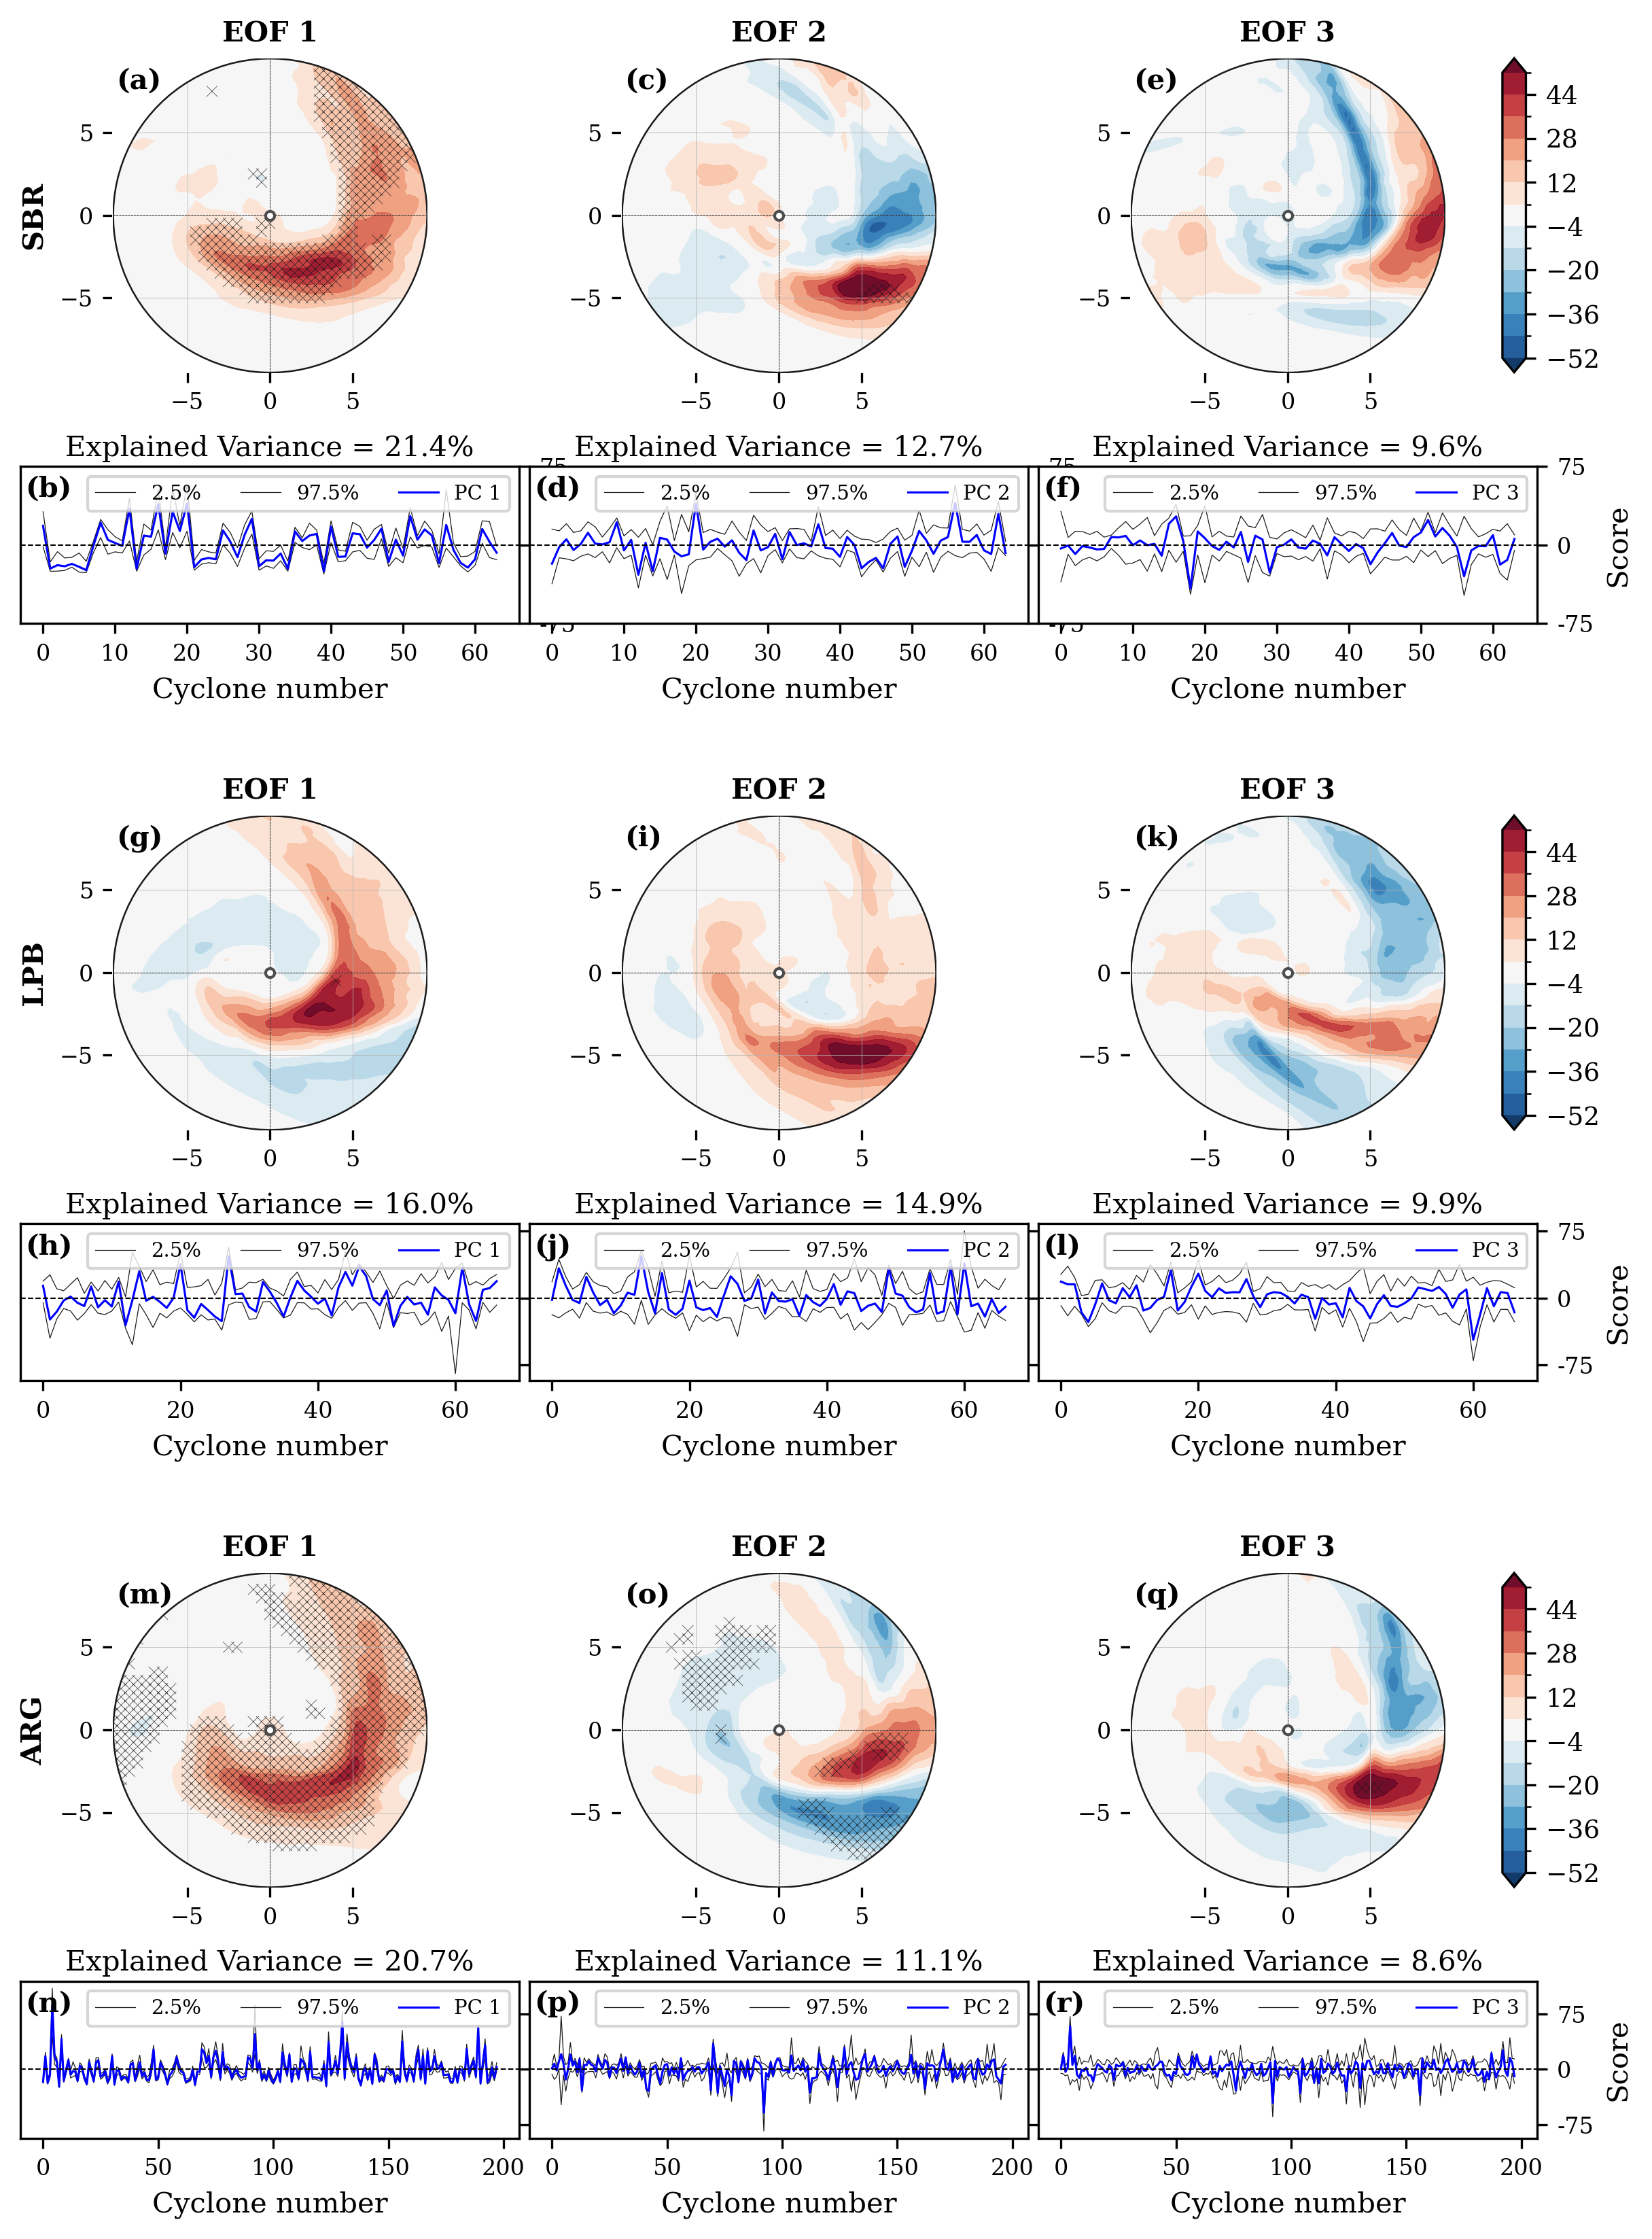
\includegraphics[width=\textwidth]{images/tp/xeof_p90_tp_mature.png}
\caption[Significância espacial dos EOFs em fase de maturidade - Subconjunto p90 (tp)]{Decomposição EOF da precipitação total para o subconjunto extremo (p90) em fase de maturidade. A disposição de painéis é idêntica à Figura~\ref{fig:xeof_madurez_global_tp}.}
\label{fig:xeof_madurez_p90_tp}
\end{figure}

A Figura~\ref{fig:xeof_madurez_global_tp} evidencia que, para a População Global em fase de maturidade, as áreas de significância estatística do EOF1 aparecem confinadas ao setor oriental do domínio, coerentes com o forçante do WCB documentado previamente. 
No entanto, diferentemente do campo de vento onde a significância abrangia domínios extensos e contíguos, aqui as zonas significativas apresentam-se fragmentadas, com manchas isoladas de achurado que não formam um padrão geométrico contínuo. 
Este aspecto visual reflete diretamente a natureza inerentemente descontínua da precipitação, onde a convecção embebida e as frentes estreitas geram sinais espaciais localizadas mas não necessariamente coerentes em escala sinóptica completa. 
As séries temporais associadas (painéis b, d, f) mostram que as flutuações de PC2 e PC3 permanecem majoritariamente dentro dos limites de confiança de 95\%, indicando que os modos secundários capturam variabilidade de menor relevância física na climatologia geral.

Pelo contrário, a Figura~\ref{fig:xeof_madurez_p90_tp} revela uma transformação qualitativa no padrão de significância. 
No subconjunto p90, e consistente com o salto na variância explicada documentado na Seção~\ref{subsec:var_exp_tp}, o EOF1 concentra suas áreas significativas em uma configuração curvada que abrange o setor sudeste e sul do domínio, traçando a geometria da banda enroscada.
Diferentemente da população global, aqui o achurado forma um arco contínuo e denso que bordeja o quadrante central, indicando que o sinal físico é estatisticamente robusto em toda a extensão da estrutura periférica. 
Notavelmente, as séries de PC2 e PC3 mostram amplitudes que em certos períodos alcançam ou superam os limites de confiança bootstrap, sugerindo que inclusive a variabilidade secundária adquire relevância física durante a transição para a decadência em sistemas severos.

Esta diferença na distribuição espacial da significância tem implicações operacionais diretas para a preditibilidade dos impactos. 
Na População Global, a fragmentação da significância indica que a localização exata dos máximos de precipitação apresenta maior incerteza espacial, respondendo à variabilidade inerente dos processos convectivos transitórios. 
No entanto, nos ciclones intensos durante a decadência, a concentração de significância na banda enroscada periférica representa um ganho de preditibilidade geométrica: a huella pluviométrica ancora-se em uma estrutura espacialmente coerente e estatisticamente replicável. 
Isto contrasta marcadamente com o comportamento observado no vento, onde a contração da significância para o núcleo em ciclones intensos indicava uma perda de preditibilidade para os flancos exteriores. 
% En el caso de la precipitación, la organización ocluida genera una firma predecible para la alerta temprana, concentrando el peligro hidrológico en sectores periféricos bien delimitados durante la fase final del ciclo de vida.

% ==============================================================================
\section{Dinâmica temporal: Componentes principais (PC1)}\label{sec:dinamica_pc1_tp}
% ==============================================================================

A fragmentação da variância documentada na fase de maturidade e sua transformação para a coerência na decadência têm sua contraparte temporal no comportamento estatístico das Componentes Principais.
O contraste entre a População Global e os ciclones intensos revela aqui uma dinâmica inversa à observada no vento: enquanto o campo cinemático mostrava um fortalecimento progressivo da correlação até a maturidade seguido de um colapso nos sistemas p90, o campo pluviométrico exibe uma assinatura correlacional invertida e distribuições de probabilidade marcadamente leptocúrticas em todos os estratos.

\subsection{População Global}\label{subsubsec:pc1_global_tp}

% TABLA 1: MOMENTOS ESTADÍSTICOS - POBLACIÓN GLOBAL
\input{tabelas_pt/tab_momentos_global_tp.tex}

% TABLA 2: CORRELACIONES - POBLACIÓN GLOBAL
\input{tabelas_pt/tab_corr_global_tp.tex}

As Tabelas~\ref{tab:momentos_global_tp} e~\ref{tab:corr_global_tp} documentam as propriedades estatísticas da primeira Componente Principal (PC1) para a População Global. 
A primeira tabela apresenta os momentos de ordem superior (viés $\gamma_1$ e curtose $\gamma_2$) que caracterizam a forma da distribuição de amplitudes do modo espacial dominante, enquanto a segunda tabela mostra os coeficientes de correlação de Pearson entre a PC1 e o mínimo de vorticidade relativa a 850 hPa ($\zeta_{850}^{min}$) alcançado por cada ciclone. 
Os valores se desagregam por região de ciclogênese e fase evolutiva, permitindo avaliar tanto a estrutura interna da variabilidade como sua relação com a intensidade dinâmica do sistema.

A análise dos momentos estatísticos revela uma característica distintiva do campo pluviométrico: a presença persistente de distribuições com caudas pesadas (leptocurtose positiva) ao longo de todo o ciclo de vida.
Diferentemente do vento, onde a curtose evoluía para valores próximos a zero ou negativos durante a maturidade, na precipitação observam-se valores de $\gamma_2$ consistentemente positivos. 
Em SBR esses valores oscilam entre $+0,87$ em intensificação e $+2,18$ em decaimento; LPB exibe curtose pronunciada em incipiência ($+2,85$) e particularmente em decaimento ($+6,02$); enquanto ARG apresenta os valores mais extremos, com curtose superiores a $+9$ tanto em incipiência como em decaimento. 
O viés positivo persistente ($\gamma_1 > +0,8$ na maioria dos casos) indica que a distribuição de amplitudes apresenta uma cauda estendida para valores altos, refletindo a presença de eventos com anomalias pluviométricas excepcionalmente intensas em relação ao padrão médio.

O exame das correlações entre PC1 e vorticidade revela um desacoplamento progressivo entre a estrutura espacial da precipitação e a intensidade rotacional do vórtice durante a maturidade nas regiões oceânicas. 
Em SBR, a correlação negativa moderada durante as fases iniciais ($\rho \approx -0,52$) inverte seu sinal na maturidade ($\rho = +0,17$, significativo) e decaimento ($\rho = +0,19$, significativo), indicando que os ciclones com maior vorticidade tendem a apresentar menores amplitudes no modo dominante de precipitação durante estas etapas. 
LPB mostra um padrão similar: correlações negativas significativas durante o desenvolvimento ($\rho = -0,49$ em incipiência, $-0,59$ em intensificação) que colapsam para valores não significativos em maturidade ($\rho = -0,04$, $p = 0,26$) e decaimento ($\rho = -0,07$, $p = 0,07$). 
Em contraste, ARG mantém correlações negativas estatisticamente significativas durante todo o ciclo, embora com enfraquecimento progressivo (de $-0,51$ em incipiência a $-0,25$ em decaimento).

Este comportamento correlacional reflete processos físicos diferenciados na evolução do ciclo de vida. 
A mudança de sinal observada em SBR e o colapso em LPB durante a maturidade respondem à divergência entre intensidade dinâmica e atividade convectiva documentada nas distribuições de probabilidade. 
Nestas regiões, os sistemas que alcançam valores extremos de vorticidade são precisamente os que desenvolvem oclusões mais completas e rápidas, onde a intrusão seca suprime a convecção profunda no domínio central lagrangiano. 
Por isso, a PC1, que captura a variação da huella pluviométrica no domínio de análise, já não escala positivamente com a profundidade do vórtice: os ciclones mais intensos dinamicamente apresentam anomalias menores no modo de precipitação porque seu núcleo se secou. 
Em ARG, a oclusão é mais lenta e o esgotamento de umidade mais gradual, o que permite manter um acoplamento residual entre vorticidade e precipitação durante mais tempo.

A variabilidade temporal destas séries de PC1, manifestada nos picos de amplitude interanual, responde a flutuações de grande escala na circulação hemisférica. 
As oscilações de baixa frequência na baroclinicidade do Hemisfério Sul, analisadas por \citet{machado2020influence}, modulam a eficiência dos sistemas ciclônicos para condensar vapor de água. 
Durante períodos de maior instabilidade baroclínica, caracterizados por cisalhamento vertical intensificado e gradientes térmicos elevados na espessura troposférica, a PC1 exibe amplitudes superiores à média, refletindo condições favoráveis para a geração de anomalias pluviométricas extremas. 
Complementarmente, \citet{simmonds2000variability} documentam ciclos temporais na profundidade e extensão dos ciclones extratropicais do Hemisfério Sul, sugerindo que os picos da série temporal de PC1 capturam janelas de maior atividade ciclogenética onde a convergência de níveis baixos se intensifica, forçando taxas de condensação superiores à População global e nos subconjunto p90.

\subsection{Subconjunto $p90$}\label{subsubsec:pc1_p90_tp}
%Leptocurtosis extrema, colapso correlacional y asimetría regional
% TABLA 3: MOMENTOS ESTADÍSTICOS - P90
\input{tabelas_pt/tab_momentos_p90_tp.tex}
% TABLA 4: CORRELACIONES - P90
\input{tabelas_pt/tab_corr_p90_tp.tex}

As Tabelas~\ref{tab:momentos_p90_tp} e~\ref{tab:corr_p90_tp} documentam as propriedades estatísticas da PC1 para o estrato de ciclones intensos. A primeira tabela apresenta a evolução dos momentos de ordem superior (viés e curtose) através das fases do ciclo de vida, enquanto a segunda tabela registra os coeficientes de correlação entre a amplitude do primeiro modo e a vorticidade mínima do sistema. 
A comparação com as tabelas correspondentes da População Global revela uma dinâmica distinta: em vez da leptocurtose persistente observada previamente, aqui documenta-se uma evolução não monotónica para valores extremos no decaimento, acompanhada de um colapso sistemático das correlações durante a fase de maturidade.

A análise das distribuições de probabilidade revela uma heterogeneização dramática do comportamento estatístico. 
Em SBR observa-se leptocurtose marcada nas fases iniciais ($\gamma_2 = +3,48$ em incipiência, $+1,67$ em intensificação), seguida de um colapso para uma distribuição quase normal na maturidade ($\gamma_2 = -0,67$) e uma explosão leptocúrtica no decaimento ($\gamma_2 = +19,77$, $\gamma_1 = +4,02$). 
LPB reproduz este padrão com valores ainda mais extremos: curtose de $+4,52$ em incipiência, evolução para simetria em maturidade ($\gamma_2 = +0,16$), e valores superiores a $+23$ em decaimento. 
ARG apresenta a curtose mais elevada do conjunto em fase incipiente ($+30,88$), mantendo valores positivos extremos durante todo o ciclo. 
Simultaneamente, as correlações com a vorticidade exibem um colapso estatístico durante a maturidade em SBR ($\rho = -0,17$, não significativo) e LPB ($\rho = -0,03$, $p = 0,80$), recuperando-se parcialmente no decaimento ($-0,34$ e $-0,50$ respectivamente), enquanto ARG mantém valores negativos significativos embora atenuados ($-0,24$ em maturidade).
A variabilidade temporal destas séries, manifestada nos pulsos de alta amplitude observados nas séries de PC1, responde às escalas características dos ciclones intensos. 
% Como evidencian \citet{chen2025characteristics}, los eventos de precipitación extrema asociados a ciclones extratropicales están dinámicamente constreñidos a periodos cortos, con escalas temporales del orden de 2 a 3 horas para las tasas máximas de condensación. 
% Esta limitación temporal explica las fluctuaciones observadas en las series de PC1: los picos pluviométricos de máxima intensidad representan inyecciones fugaces de ascensos térmicos embebidos en el ciclo de vida sinóptico de los ciclones, generando la cola pesada que caracteriza a las distribuciones del estrato p90.

O colapso correlacional durante a maturidade em SBR e LPB constitui o correlato temporal do desacoplamento espacial documentado nas análises de PDF e KDE. 
Quando alcançam sua máxima profundidade dinâmica, a precipitação no domínio deixa de ser governada pela intensidade rotacional do sistema para depender da geometria específica da oclusão. 
A posição da banda enroscada em relação ao centro do domínio determina a presença ou ausência de anomalias positivas na PC1, introduzindo variabilidade que não correlaciona linearmente com a vorticidade. 
Isto explica a evolução para a normalidade estatística na maturidade seguida da explosão leptocúrtica no decaimento: à medida que os sistemas se dissipam, alguns retêm a banda enroscada dentro do domínio (gerando a cauda positiva extrema), enquanto outros a deslocaram para o exterior.
Este desacoplamento obedece a uma reestruturação termodinâmica impulsionada por retroalimentações locais de mesoescala. 
% Durante el análisis del evento severo Raoni en el Atlántico Sur, \citet{reboita2022from} documentan cómo los flujos turbulentos de superficie alimentan convección vigorosa que redistribuye la vorticidad potencial mediante liberación masiva de calor latente. 
Este aquecimento diabático reduz o cisalhamento vertical e consolida a seclusão quente, desacoplando a dinâmica da precipitação periférica das flutuações lineares do gradiente sinóptico de fundo, conferindo aos ciclones maduros uma evolução quase independente em relação à intensidade do ciclone.

A alteração da estrutura vertical da vorticidade potencial durante a maturidade rompe a linearidade entre campos de superfície e dinâmica de grande escala. 
% Según \citet{crespo2020potential}, la evolución de los ciclones en el este de Sudamérica está ligada a la interacción entre anomalías de vorticidad potencial en la alta troposfera y el calentamiento diabático en niveles bajos. 
% En ciclones intensos, la liberación masiva de calor latente asociada a las precipitaciones enroscadas genera profundas anomalías de vorticidad potencial en la baja troposfera que dominan la circulación local, rompiendo la relación lineal con el gradiente de presión de fondo y propiciando la bifurcación estructural observada en las series.
A persistência de correlações significativas em ARG durante toda a evolução reflete uma dinâmica de oclusão diferenciada. 
Nesta região, os ciclones desenvolvem oclusões mais lentas e heterogêneas, com intrusão seca menos violenta que nas regiões oceânicas. 
A modulação orográfica da cordilheira dos Andes e o controle da umidade por advecção zonal, em vez de intercâmbio oceânico, geram um acoplamento mais persistente entre vorticidade e precipitação, embora atenuado em relação às fases iniciais. 
Isto explica por que em ARG a PC1 nunca perde completamente sua correlação com a intensidade dinâmica, mantendo valores significativos inclusive durante a maturidade.

Estes resultados demonstram que o campo de precipitação é estruturalmente mais complexo que o cinemático. A combinação de distribuições, correlações que colapsam e recuperam, e diferenças regionais marcadas indica que parametrizar a precipitação utilizando unicamente a vorticidade resulta inadequado, particularmente durante a fase crítica de maturidade nas regiões oceânicas onde o desacoplamento é mais pronunciado.

% ==============================================================================
\section{Síntese}\label{sec:sintesis_tp}
% ==============================================================================

A análise do campo de precipitação total revela uma arquitetura que evolui desde um regime de dispersão frontal para um de concentração ocluída, dependendo criticamente da intensidade dinâmica do sistema. 
Na população global, a precipitação organiza-se como uma resposta assimétrica ao forçante do WCB: as distribuições de probabilidade exibem caudas pesadas persistentes (viés positivo e leptocurtose), os máximos concentram-se no quadrante oriental do domínio, e a variância espacial distribui-se entre múltiplos modos sem que o EOF1 domine. 
Esta configuração reflete que, no regime médio, a chuva está governada pela disponibilidade de umidade ambiental e pela convergência frontal transitória do WCB, sem uma dependência linear com a vorticidade, como confirmam as correlações fracas ou inexistentes entre PC1 e vorticidade durante a maturidade em SBR e LPB.

Em contraste, os ciclones intensos (p90) exibem uma arquitetura pluviométrica qualitativamente diferente que emerge da transição para a oclusão. A reorganização espacial observada no KDE e o salto na variância explicada pelo EOF1 (do 11--16\% típico ao 36,5\% em LPB durante o decaimento) respondem primariamente ao processo de oclusão ao estilo Shapiro-Keyser. A intrusão seca profunda aniquila a convecção no núcleo central e confina a umidade remanescente em uma banda periférica enroscada.
% (\textit{wrap-around precipitation}) morfológicamente coherente \citep{schultz2021antecedents}. 
Este processo gera o colapso das PDF para modas de baixa precipitação central simultâneo ao pico de ventos destrutivos, confirmando o desacoplamento temporal entre forçantes cinemático e hidrológico nos eventos mais severos.

A superposição dos campos de vento e precipitação nos ciclones intensos — cuja huella eólica assimétrica foi quantificada independentemente no Capítulo~\ref{cap:resultados_wind10} — evidencia geometricamente o desacoplamento espacial dos perigos. 
Enquanto os ventos máximos se hiperconcentram no quadrante noroeste associados à cinta transportadora fria, os máximos pluviométricos remanescentes organizam-se em uma ferradura sólida no sudeste e sul, orbitando a margem da intrusão seca. 
Esta configuração opera sob o marco conceitual de eventos compostos, onde os perigos surgem da combinação de múltiplos processos físicos interagindo a diferentes escalas \citep{zscheischler2018future}. 
No Atlântico Sudoeste, isto implica que as ameaças mais severas por inundações relâmpago ocorrerão preferentemente durante as etapas de gênese e intensificação quando o acesso à umidade tropical é ativo.

As diferenças regionais modulam esta arquitetura geral mediante a interação com as condições de superfície. 
Em SE-BR e LPB, os fluxos de calor latente oceânico e o jato de camadas baixas favorecem o desenvolvimento do desacoplamento mais pronunciado entre vorticidade e precipitação, enquanto em ARG a modulação orográfica e oclusões mais lentas geram um regime de transição mais gradual entre dinâmica e umidade, como reflete a persistência de correlações significativas nesta região \citep{marrafon2022classificacao}. 
Esta multiplicidade de vias evolutivas, onde a termodinâmica do núcleo determina a organização espacial final, explica a coexistência de distribuições heterogêneas entre regiões ao longo do ciclo de vida.

O estabelecimento desta base hidrometeorológica — em particular a demonstração estatística do desacoplamento espaço-temporal entre vento e chuva em eventos severos — provê o alicerce teórico para a análise combinada mediante Funções Ortogonais Empíricas Multivariadas (MEOF) no capítulo seguinte, onde se explorará explicitamente a covariância conjunta de ambos os campos de vento e precipitação.